\RequirePackage{lineno} % Numeração de linhas para revisão.
\documentclass[a4paper,11pt]{article} % Classe do documento como artigo, tamanho A4 e fonte 11pt.
\usepackage{fancyhdr} % Personalização de cabeçalhos e rodapés.
\fancyhf{} % Limpa cabeçalhos e rodapés anteriores.
\setlength{\headheight}{13.59999pt} % Define a altura do cabeçalho.
\usepackage[utf8]{inputenc} % Codificação UTF-8 para caracteres especiais.
\usepackage[brazil]{babel} % Configurações para o português do Brasil.
\usepackage{graphicx} % Inclusão de gráficos e imagens.
\usepackage{latexsym,amssymb,amsmath,amsfonts} % Símbolos e fontes da AMS para matemática.
\usepackage[left=2.5cm, right=2.5cm, top=2.5cm,bottom=2.5cm]{geometry} % Define as margens do documento.
\usepackage{url} % Formatação correta de URLs.
\usepackage{indentfirst} % Indenta o primeiro parágrafo de cada seção.
\usepackage{enumerate} % Personalização de listas enumeradas.
\usepackage[ocgcolorlinks]{hyperref} % Links clicáveis com cores que não afetam a impressão.
\usepackage{comment} % Inclusão/exclusão de blocos de texto.
\usepackage{lipsum} % Texto gerado automaticamente para preenchimento.

\usepackage{courier} % Fonte Courier New
\usepackage{subcaption}
\usepackage{float}

\begin{document}
%%%%%%%%%%%%%%%%%%%%%%%%%%%%%%%%%%%%%%%%%%%%%%%%%%%%%%%%%%%%%%%%%%%%%%%%%%%%%%%%%%%%%%%%%%%%%%%%%%%%%
\pagestyle{fancy}
\setcounter{page}{1}
\renewcommand{\thefootnote}{$\dagger$}
\lhead{ISSN: 2317-0840 }
\lfoot{}
\cfoot{\small \slshape {\bf Sigmae}, Alfenas, v.xx, n.x, p. x-x, 20xx.} % Informações do rodapé
\rfoot{}
\setpagewiselinenumbers
\modulolinenumbers[1]
\linenumbers
%%%%%%%%%%%%%%%%%%%%%%%%%%%%%%%%%%%%%%%%%%%%%%%%%%%%%%%%%%%%%%%%%%%%%%%%%%%%%%%%%%%%%%%%%%%%%%%%%%%%

\begin{center}
    {\large {\bf Comparação e Desempenho dos Testes de Normalidade Implementados na Linguagem de Programação R via Simulação de Monte Carlo}}\vspace{0.3cm}
\end{center}

\begin{small}

\noindent{\bf Resumo:} {\it 
    O objetivo deste trabalho foi avaliar as taxas de erro tipo I e poder dos testes de normalidade kolmogorov-Smirnov (KS), Shapiro-Wilk (SK), Anderson-Darling (AD), D’Agostinho-Pearson (DP), Lilliefors (LF), Jarque-Bera (JB), Crámer-Von-Mises (CVM) implementados na linguagem de programação $R_{4.4.1}$ for windows para decidir quais apresentam o melhor desempenho. A metodologia utilizada foi um estudo de Simulação de Monte Carlo, que utilizou as distribuições (Normal, beta e gama) e cinco tamanhos de amostras foram simuladas 1.000 amostras de cada par distribuição-tamanho e realizado os testes. Sob normalidade, os testes foram exatos e, em relação ao poder, o desempenho foi afetado pelo tamanho da amostra e tipo de distribuição. Para amostras grandes, maiores que 500, o teste \textit{Zhang(2002)} apresentou o melhor desempenho e no caso de amostras pequenas, de uma maneira geral, o teste Shapiro-Wilk obteve os melhores resultados. Aplicou-se o teste Kappa-Fleis para avaliar a concordância na tomada de decisão. Para a maioria das distribuições, os testes tiveram forte concordância; Os testes de KS e AD se mostraram muito pouco poderoso, mesmo para grandes amostras.}\vspace{0.3cm}

\noindent{\bf Palavras-chave:} {\it Normalidade; Monte Carlo; Erro Tipo I; Shapiro-Wilk; kolmogorov-Smirnov.}\vspace{0.3cm}

\end{small}

\begin{center}
    {\large {\bf Comparison and Performance of Normality Tests Implemented in the R Programming Language via Monte Carlo Simulation}\vspace{0.3cm}}
\end{center}

\begin{small}

\noindent{\bf Abstract:} {\it 
    The aim of this study was to evaluate the Type I error rates and power of the normality tests Kolmogorov-Smirnov (KS), Shapiro-Wilk (SW), Anderson-Darling (AD), D'Agostino-Pearson (DP), Lilliefors (LF), Jarque-Bera (JB), and Crámer-Von-Mises (CVM) implemented in the R programming language to determine which ones perform best. The methodology used was a Monte Carlo Simulation study, which employed the following distributions: Normal, Beta and Gamma. For five sample sizes, 1,000 samples were simulated for each distribution-size pair, and the tests were performed. Under normality, the tests were accurate, and regarding power, performance was influenced by sample size and distribution type. For large samples, greater than 500, the \textit{Zhang(2002)} test showed the best performance, while for small samples, the Shapiro-Wilk test generally produced the best results. The Fleiss' Kappa test was applied to assess agreement in decision-making. For most distributions, the tests demonstrated strong agreement; however, the KS and AD tests proved to be very low in power, even for large samples.}\vspace{0.3cm}

\noindent{\bf Keywords:}  {\it Normality; Monte Carlo; Type I Error; Shapiro-Wilk; Kolmogorov-Smirnov).\vspace{0.3cm}}

\end{small}
%%%%%%%%%%%%%%%%%%%%%%%%%%%%%%%%%%%%%%%%%%%%%%%%%%%%%%%%%%%%%%%%%%%%%%%%%%%%%%%%%%%%%%%%%%%%
\newpage                                                                                   
\pagestyle{fancy}                                                                          
\renewcommand{\thefootnote}{\roman{footnote}}                                              
\lhead{}
\chead{\small \slshape}
\rhead{\thepage}
\lfoot{}
\cfoot{\small \slshape {\bf Sigmae}, Alfenas, v.xx, n.x, p. x-x, 20xx.}
\rfoot{}

%%%%%%%%%% 1. Introdução %%%%%%%%%%
\section{Introdução}

De acordo com Dufour et al. (1998), aproximadamente 40 testes de normalidade estão disponíveis, frequentemente gerando resultados opostos para o mesmo conjunto de dados, ao rejeitar ou não a hipótese de normalidade. Essa disparidade decorre das diferentes abordagens e métodos de verificação empregados por cada teste, bem como da variedade infinita de possíveis amostras. Consequentemente, a eficácia de cada teste pode variar dependendo da amostra analisada. Diante dessa diversidade, o objetivo é comparar diversos testes em diferentes cenários para determinar qual deles apresenta melhor desempenho em cada caso.\vskip0.3cm

De modo geral, muitos métodos estatísticos requerem que os dados sigam uma distribuição normal, além de pressupor independência entre as observações. Isso levanta a questão: como podemos verificar se a distribuição dos dados em análise se aproxima de uma distribuição normal?\vskip0.3cm


Duas formas de avaliar o desempenho de um teste é analisar as \textbf{Taxas de Erro Tipo I}, sob hipótese nula ($H_0$), e por meio do \textbf{Poder do Teste}, simulando-se dados sob a hipótese alternativa ($H_1$). \vskip0.3cm

Nesse contexto, o objetivo do trabalho foi avaliar as taxas de erro tipo I e poder dos testes de normalidade implementados na linguagem de programação \textbf{\textit{R 4.4.1}} (R CORE TEAM, 2023) e um ambiente de desenvolvimento integrado chamado \textbf{Rstudio} \textit{versão 1.12}, para decidir quais apresentam o melhor desempenho.


%\newpage
\section{Referencial Teórico}
\subsection{A Distribuição Normal}

Para o estudo de simulação é necessário definir uma das mais importantes  variáveis aleatórias contínuas, chamada distribuição normal, sendo que a maioria dos fenômenos aleatórios pode ser descrita de forma aproximada por ele.\vskip0.3cm

Seja $X$ uma variável aleatória que assume todos os valores reais $- \infty < x < +\infty$, tem distribuição normal (ou gaussiana) com média $\mu$ e  variância $\sigma$, se sua função densidade de probabilidade (fdp) é dada por (MEYER, 1987):

\begin{equation}
f(x) = \frac{1}{\sqrt{2 \pi \sigma}} \exp \left(-\frac{1}{2} \left[\frac{x- \mu}{\sigma} \right]^{2} \right) \ , \ - \infty < x < +\infty
\end{equation}

Os parâmetros  $\mu$ e $\sigma$ devem satisfazer às condições  $-\infty < \mu < +\infty$ e $\sigma^{2} > 0$. Denotamos esta distribuição por $X \backsim N(\mu, \sigma^{2})$



\subsection{Testes de Normalidade}

A seguir serão apresentados os testes de normalidade selecionados para realização da simulação de Monte Carlo. Foram selecionados vários testes para este estudo. Dentre estes testes, tem-se \textit{testes clássicos}, como Shapiro-Wilk, Kolmogorov-Smirnov, etc. e \textit{testes modernos}, propostos por Zhang (2002).\vskip0.3cm

Com o objetivo de encontrar o mais adequado e poderoso teste de aderência à distribuição Normal, em função de diferentes tamanhos amostrais.

\subsubsection{kolmogorov-Smirnov}

O teste de kolmogorov-Smirnov é uma referência aos matemáticos russos \textbf{Andrey kolmogorov} e \textbf{Vladimir Ivanovich Smirnov}. Este é uma prova de bondade de ajuste para dados contínuos, o quanto a amostra provem de uma população com uma determinada distribuição teórica. Especificando quanto a distribuição de frequência acumulada observada se aproxima da distribuição aacumulada teórica.\vskip0.3cm

O teste de kolmogorov-Smirnov foi aplicado usando a função \texttt{ks.test()} do pacote \textit{stats}. \vskip0.3cm

\subsubsection{Lilliefors}

Lilliefors (1967) propôs modificar os parâmetros do teste de kolmogorov-smirnov para simplificar os cálculos e resolver a limitação utilizando estimativas populacionais da média e desvio-padrão.\vskip0.3cm

A estatística do teste é:

\begin{equation}
   D = max_{(i=1,...,n)}|D^{+},D^{-}|
\end{equation}

Sendo

\begin{equation}
    D^{+} =   \underbrace{max}_{\mbox{i=1,...,n}}    {\left[\frac{i}{n} - p_{(i)}\right]} \ \ e \ \ D^{-} = \underbrace{max}_{\mbox{i=1,...,n}}  {\left[p_{(i)} - \frac{i-1}{n}\right]}
\end{equation}

$ p_{(i)}= \phi( \frac{x_{(i)-\Bar{x}}}{s} )$, sendo $\phi$ a função de distribuição acumulada normal padrão, com x e s, respectivamente, a média e o desvio padrão amostral dos dados.\vskip0.3cm


O valor p é calculado a partir da fórmula de Dallal-Wilkinson (1986), com base na estatística modificada:

\begin{equation}
    Z = D \left[(\sqrt{n} - 0.01) + \frac{0.85}{\sqrt{n}} \right]
\end{equation}


\vskip0.3cm


Para o teste de Lilliefors, a função do R é a \texttt{lillie.test()} do pacote \textit{nortest} que nos fornece as mesmas informações dos outros testes, a estatística do teste e o valor-p.\vskip0.3cm






\subsubsection{Anderson Darling}

Anderson e Darling (1952) sugeriram um teste de normalidade baseado na função de distribuição empírica, para distribuições com parâmetros conhecidos, definido como: 

\begin{equation}
    A = -n - \frac{1}{n} \sum_{i=1}^{n} [(2i-1)[ \ln (p_{(i)}) + \ln(1- p_{(n-1+i)})]
\end{equation}

Em que $p_{(i)}$ são os percentis ordenados da distribuição normal padrão, $\phi$ é a função de distribuição acumulada nomal padrão, x é a média amostral e s é o desvio padrão amostral.\vskip0.3cm

O cálculo do p-valor foi proposto posteriormente, por Stephens (1986), e é encontrado através da fórmula estatística ajustada,

\begin{equation}
    Z = A \left[ \left(1.0 + \frac{0.75}{n} \right)+  \left(n+\frac{2.25}{n^{2}} \right) \right]
\end{equation}


No R a função \texttt{ad.test()} do pacote \textit{nortest} fornece a estatística de teste e o p-valor. \vskip0.3cm

\subsubsection{Shapiro Wilk}

O teste proposto por Shapiro e Wilk (1965) é considerado mais sensível para diversas distribuições, no R foi a função \texttt{shapiro.test()} do pacote \textit{nortest} fornece a estatística teste e o valor-p. Para verificar se uma amostra segue uma distribuição normal, utiliza-se a seguinte estatística de teste: 

\begin{equation}
    SW = \frac{\sum_{i=1}^{n} (a_{i}y_{i})^{2}}{\sum_{i=1}  (y_{i} - \bar{y})^{2}}
\end{equation}

em que $y_{i}$ é o o-ésimo valor da amostra observada, $\hat{y}$ é a média amostral e $a_{i},a_{2},...,a_{n}$ são constantes calculada da seguinte forma:

\begin{equation}
    (a_{1},a_{2},...,a_{n})^{T} = \frac{m^{T}V^{-1}}{(m^{T}V^{-1}V^{-1} )^{1/2}}
\end{equation}

sendo $m=(m_{1},m_{2},...,m_{n})^{T}$ o vetor de valores esperados das estatísticas de ordem da amostra e $V$ é a matriz das covariâncias desta estatística.\vskip0.3cm

\subsubsection{D’Agostino-Pearson}

O teste de D'Agostino-Pearson utiliza as estatísticas de assimetria (Skewness) e curtose (Kurtosis) para verificar a normalidade. A fórmula envolve calcular ambas as medidas e combiná-las em uma estatística conjunta (D'AGOSTINO \& PEARSON, 1973).\vskip0.3cm

Com isso, a primeira parte da fórmula a seguir mede o grau de $\textbf{assimetria}$ dos dados (\textit{skewness}):

\begin{equation}
g_{1} = \frac{\sqrt{n(n-1)}}{n-2} \times \frac{\sum_{i1}^{n} (x_{i}-\bar{x})^{3}}{\left( \sum_{i=1}^{n} (x_{i}-\bar{x})^{2}\right)^{3/2}}
\end{equation}

Com relação a segunda parte da fórmula, mede o grau de achatamento($\textbf{curtose}$) ou pico da distribuição dos dados:

\begin{equation}
g_{2} = \frac{n(n+1)}{(n-1)(n-2)(n-3)} \times \sum_{i=1}^{n} \left(  \frac{(x_{i}-\bar{x})^{4}}{s^{4}} \right) - \frac{3(n-1)^{2}}{(n-2)(n-3)}
\end{equation}

onde, $n$ é o tamanho da amostra, $\bar{x}$ é a média da amostra, $x_{i}$ são os valores individuais da amostra e $s$ é o desvio padrão da amostra.\vskip0.3cm

A estatística do teste  D'Agostino-Pearson é a soma das estatísticas z-normalizadas de assimetria ($G_{1}$) e curtose ($G_{2}$):\vskip0.3cm

\begin{equation}
    K^{2} = Z_{1}^{2}(g_{1}) + Z_{2}^{2}(g_{2})
\end{equation}

O valor de $K^{2}$ segue uma distribuição qui-quadrado com 2 graus de liberdade. Se for maior que o valor crítico da distribuição qui-quadrado, rejeita-se a hipótese nula de que a amostra segue uma distribuição normal.\vskip0.3cm

NO que tante ao teste de D’Agostino-Pearson foi usada a função \texttt{agostino.test()} pertencente ao pacote \textit{moments}.\vskip0.3cm


\subsubsection{Cramér-Von Mises}

O teste de Cramér-von Mises é uma alternativa ao teste de Kolmogorov-Smirnov, pois
apesar de ambos avaliarem as diferenças entre as distribuições empírica e teórica, a estatística de teste é calculada de outra maneira.\vskip0.3cm

Este teste foi proposto por Harold Cramér e Richard Von Mises, em 1928. Porém, algumas modificações foram criadas. Darling (1957) definiu a estatística teste da seguinte forma:

\begin{equation}
    W = \frac{1}{12n} + \sum \left[ p_{(i)} - \frac{2i-1}{2n} \right]^{2}
\end{equation}

onde $n$ é o tamanho amostral, $p_{i} = \phi \left(  \frac{x_{i}-\bar{x}}{s} \right)$, $\phi$ é a função de distribuição acumulada normal padrão, com $\bar{x}$ e $s$, respectivamente, a média e o desvio-padrão amostral.\vskip0.3cm

O cálculo do p-valor foi proposto posteriormente, por Stephens (1979), e é encontrado através da fórmula estatística,

\begin{equation}
    Z = W \left(1 + \frac{0.5}{n} \right)
\end{equation}

A função \texttt{cmv.test()} do pacote \textit{nortest} foi usada para o teste de Cramér-Von Mises, fornecendo a estatística e o valor-p.\vskip0.3cm

\subsubsection{Jarque-Bera}

Em relação ao Teste de Jarque-Bera foi utilizado a função  \texttt{JarqueBeraTest()} do pacote \textit{DescTools}. Este teste foi proposto por Jarque e Bera (1980) e baseia-se na diferença entre a simetria e a curtose dos dados amostrais e teóricos da distribuição normal. A estatística do teste é definida como: 

\begin{equation}
    JBR = \frac{n}{C_{1}} \left( \frac{\hat{\mu_{3}}}{J^{3}_{N}}  \right)^{2} + \frac{n}{C_{2}} \left( \frac{ \hat{\mu_{4}}}{J^{4}_{N}} - 3 \right)^{2} 
\end{equation}


em que $\mu_{k} = \sum_{i=1}^{n} (x_{i}- \Bar{x})^{k}$, $J_{n} = \sqrt{\frac{\pi}{2}}\frac{\sum_{i=1}^{n}|x_{i}-M|}{n}$, já M é a mediana dos valores de $x_{i}$ da amostra e $C_{1}$ e $C_{2}$ são constantes positivas que podem ser obtidas através de simulação via Monte Carlo. \vskip0.3cm

\subsubsection{Zhang(2002)}

Em 2002, Zhang apresentou 3 novos testes de normalidade, baseados na função de distribuição empírica, no qual modifica os parâmetros dos testes tradicionais de Anderson-Darling, Cramér-Von Mises e kolmogorov-Smirnov e cria três testes($Z_{A}, Z_{C}$ e $Z_{K}$) adaptados para aderência a normalidade.\vskip0.3cm

Nesse contexto, são fornecidos novos tipos de testes para normalidade, abrangentes que geralmente são muito mais poderosos que os testes tradicionais. \vskip0.3cm

Assim, a nova estatística chamada $Z_{A}$ semelhantes à estatística do teste de Anderson-Darling, é definida como:

\begin{equation}
    Z_{A} = - \sum_{i=1}^{n} \left\{  \frac{ \ln[F_{0}(X_{(i)})]}{(n-i)+0.5} + \frac{1-F_{0}(X_{(i)})}{i-0.5}  \right\}  
\end{equation}

A próxima estatistica de teste $Z_{C}$, é muito pareceida à estatística do teste de Cramer-Von Mises, é apresentada como:

\begin{equation}
    Z_{C} = \sum_{i=1}^{n}  \left\{ \ln\left[ \frac{F_{0}(X_{(I)})^{-1}-1}{(n-0.5)/(i-0.75)-1} \right] \right\}
\end{equation}

A terceira estatística de teste definida como $Z_{K}$, similar à estatística do teste de Kolmogorov-Smirnov, é definida como:

\begin{equation}
Z_{K} = \underbrace{max}_{\mbox{i=1,...,n}} \left\{(i - 0,5) \ln\left[ \frac{i - 0,5}{n F_{0}(X_{(i)})} \right] + (n - i + 0,5) \ln\left[ \dfrac{(n - i) + 0,5}{n[1 - F_{0}(X_{(i)})]} \right] \right\}
\end{equation}

Em 2020, Cui e Zhou, criaram o pacote na linguagem de programação R chamado \textit{DistributionTest}, possibilitando o cálculo dos teste propostos por Zhang(2002). Com isso,  utilizou-se as funções: \texttt{za.test()}, \texttt{zc.test()} e \texttt{zk.test()} para aplicação das referidas estatísticas de teste. \vskip0.3cm

%Zhang, J.; Wu, Y. Testes de razão de verossimilhança para normalidade. Comput. Stat. Dados Anal. 2005 , 49 , 709–721



%%%%%%%%%% 2. Materiais e Métodos %%%%%%%%%%
\section{Materiais e Métodos}
A Simulação de Monte Carlo foi utilizada para simular amostras normais sob a hipótese nula de normalidade, $H_0$, para avaliar as taxas de erro tipo I dos testes e amostras sob a hipótese alternativa, $H_1$, ou seja, dados de distribuições não normais para avaliar o poder. Para cada cenário, os testes de normalidade foram aplicados ao nível de significância pré-estabelecido de $\alpha = 5\%$. \vskip0.3cm

Caso tenha sido rejeitada a hipótese nula e a amostra tenha sido gerada da distribuição normal, foi cometido um erro do tipo I. Da mesma forma se a hipótese nula for rejeitada e a amostra foi obtida de uma população não-normal, uma decisão correta foi tomada. Não foi considerado o cenário de simulação gerando distribuições com a presença de outliers. As distribuições foram simuladas por meio das funções \textit{random} do pacote base do R.

\subsection{Simulação de Monte Carlo}
Neste estudo, a eficácia dos testes de normalidade foi avaliada por meio da simulação de distribuições tanto normais quanto não normais, abrangendo casos simétricos e assimétricos, como Normal, Uniforme, Beta, t-Student, Cauchy e Exponencial. Foram considerados seis tamanhos de amostra distintos para cada distribuição: 30, 50, 100, 300, 500 e 1000. Em cada caso, foram realizadas 1.000 replicações, durante as quais os p-valores dos testes de normalidade foram registrados para análise posterior. \vskip0.3cm

%O desempenho dos seguintes testes de aderência aplicado no software R foi avaliado. 














\subsection{Erro Tipo I}
Foram simuladas 1000 amostras aleatórias da distribuição Normal com média 0 e desvio-padrão 1, $Normal(0, 1)$, utilizando a função \texttt{rnorm()} do pacote base do R. Após a aplicação dos testes de normalidade, se a hipótese de normalidade foi rejeitada a um nível nominal de significância de 0.05, os dados foram erroneamente considerados como não normais, resultando em taxas de erro tipo I. \vskip0.3cm

A proporção de rejeições incorretas foi calculada para cada teste, permitindo a identificação de testes conservadores ou liberais com base na comparação com o nível de significância $\alpha$.

\subsection{Teste de Kappa de Concordância}
Foi conduzida uma análise estatística em que os dados foram agrupados em diferentes distribuições com tamanhos de amostra variados. Utilizou-se o teste Kappa-Fleiss (descrito por CONGER, 1980) através da função \texttt{Kappam.fleiss()} do pacote \textit{irr}, com o objetivo de avaliar o nível de concordância entre os testes de normalidade empregados na decisão de aceitar ou rejeitar a hipótese nula de normalidade. \vskip0.3cm

Esta avaliação de concordância foi realizada exclusivamente para amostras que não apresentaram distribuição normal. O foco da análise foi verificar se o poder dos testes influencia diretamente na concordância entre eles.


%\newpage
%%%%%%%%%% 2. Resultados e Discussão %%%%%%%%%%
\section{Resultados e Discussão}
Os resultados serão apresentados de acordo com as taxas de erro tipo I, na situação de distribuição normal, e poder, na situação de outras distribuições. Na figura 1 estão representadas as taxas de erro tipo I dos testes de normalidade Anderson-Darling (AD), Crámer-Von-Mises (CM), D’Agostino-Pearson (DG), Jarque-Bera (JB), Kolmogorov-Smirnov (KS), Lilliefors (LL), Shapiro-Wilk (SW) e Zhang (Za, Zc, Zk) para diferentes tamanhos amostrais. \vskip0.3cm

Todos os testes apresentaram taxas de erros próximas de 0,05 sendo, por isso, considerados exatos, com a exceção dos testes de Anderson Darling e Kolmogorov-Smirnov. \vskip0.3cm

Seus valores ficarm dentro do IC para proporções (\textit{p}) construídos a 99\% de confiança com $\alpha = 0.05, IC_{99\%}(p): [0.02279;0.0654].$
\vskip0.3cm

Segundo Thode Junior (2002), em resultados de simulação observou-se que, os testes de kolmogorov-smirnov e Qui-quadrado possuem poder tão baixo que deveriam ser desconsiderados como testes de normalidade.\vskip0.3cm

Foi desenvolvido um script na linguagem de programação R, para auxiliar nos cálculos da simulação de Monte Carlo armazenado no repositório \textit{Github} que pode ser acessado no seguinte link: \href{https://github.com/MarioDhiego/Teste\_Normalidade}{https://github.com/MarioDhiego/Teste\_Normalidade}

\vskip0.3cm


De acordo com a tabela X, os resultados do teste de kappa para diferentes distribuições descritas anteriormente, percebe-se que, para a maioria das distribuições, os testes tiveram forte concordância entre rejeitar ou não a hipótese de normalidade. 



\begin{table}[H]
\centering
 \begin{tabular}{c|c}
\hline \hline
Distribuição de Probabilidade  &  Teste de kappa-Fleiss\\
\hline
      Normal(0,1)              &  \\
      Beta(2,5)                &  \\
      Cauchy(0,1)              &  \\
\hline \hline
    \end{tabular}
    \caption{Teste kappa-Fleiss de Concordância para os testes de normalidade.}
    \label{tab:my_label}
\end{table}




\newpage
%%%%%%%%%% Erro Tipo I -> Distribuição Normal %%%%%%%%%%
\begin{figure}[H]
    \centering
    \caption{Comparação do Erro Tipo I dos testes AD, CM, DG, LL, JB, KS, LL, ZA, ZC e ZK em função do tamanho amostral para a \textbf{Distribuição} \(\textbf{Normal}(0, 1)\).}
    \label{fig:erro_tipo_I_dist_norm}
    
    % Primeira linha
    \begin{subfigure}[b]{0.45\textwidth}
        \centering
        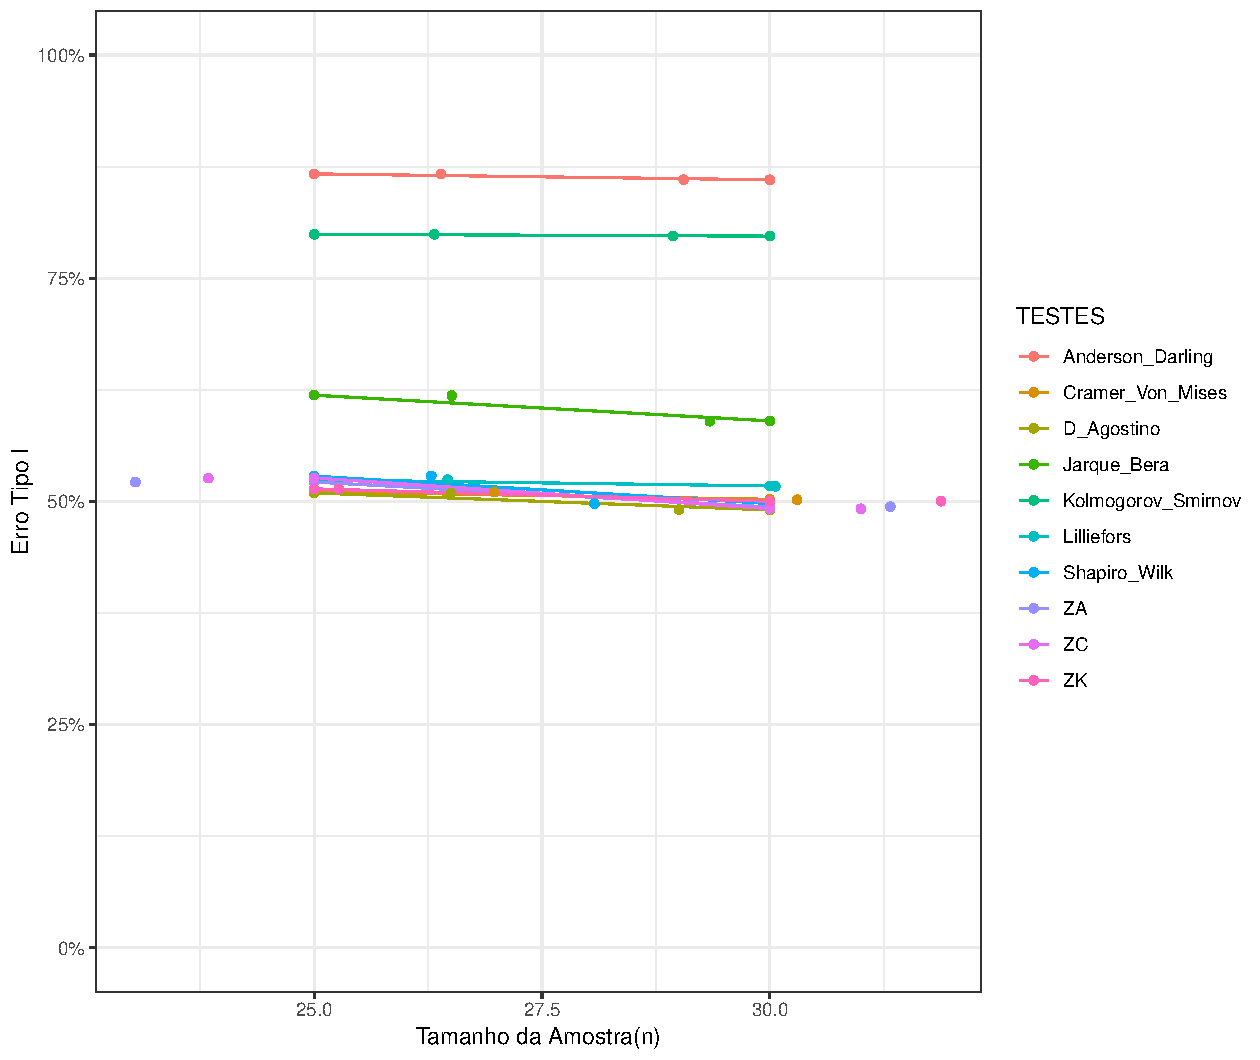
\includegraphics[width=\textwidth]{Distribuição Normal/Erro Tipo I/erro_tipo_I_normal_30.pdf}
        \caption{Tamanho amostral \(n = 30\)}
        \label{fig:normal_30}
    \end{subfigure}
    \hfill
    \begin{subfigure}[b]{0.45\textwidth}
        \centering
        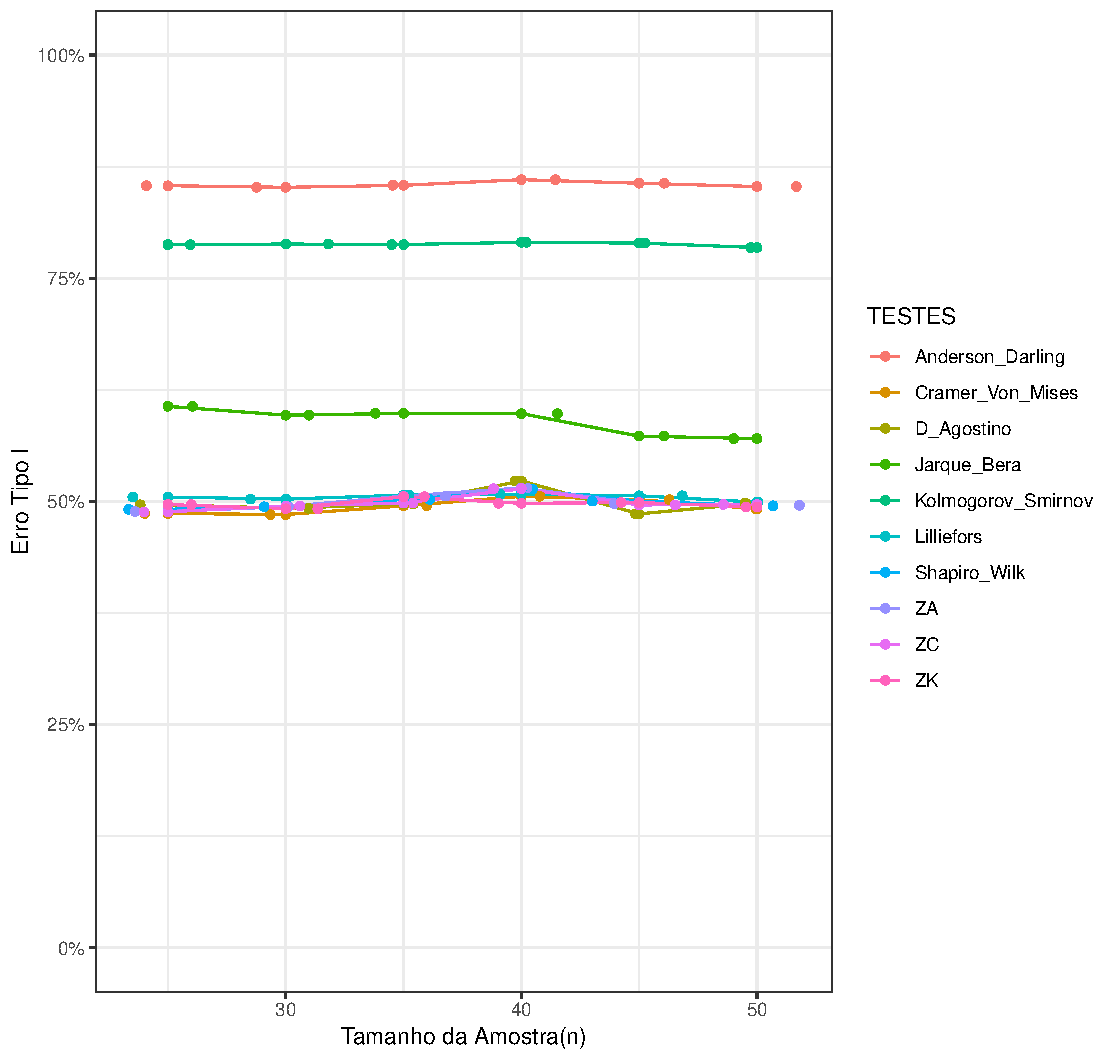
\includegraphics[width=\textwidth]{Distribuição Normal/Erro Tipo I/erro_tipo_I_normal_50.pdf}
        \caption{Tamanho amostral \(n = 50\)}
        \label{fig:normal_50}
    \end{subfigure}
    
    % Segunda linha
    \vspace{0.5cm} % Espaçamento entre linhas
    \begin{subfigure}[b]{0.45\textwidth}
        \centering
        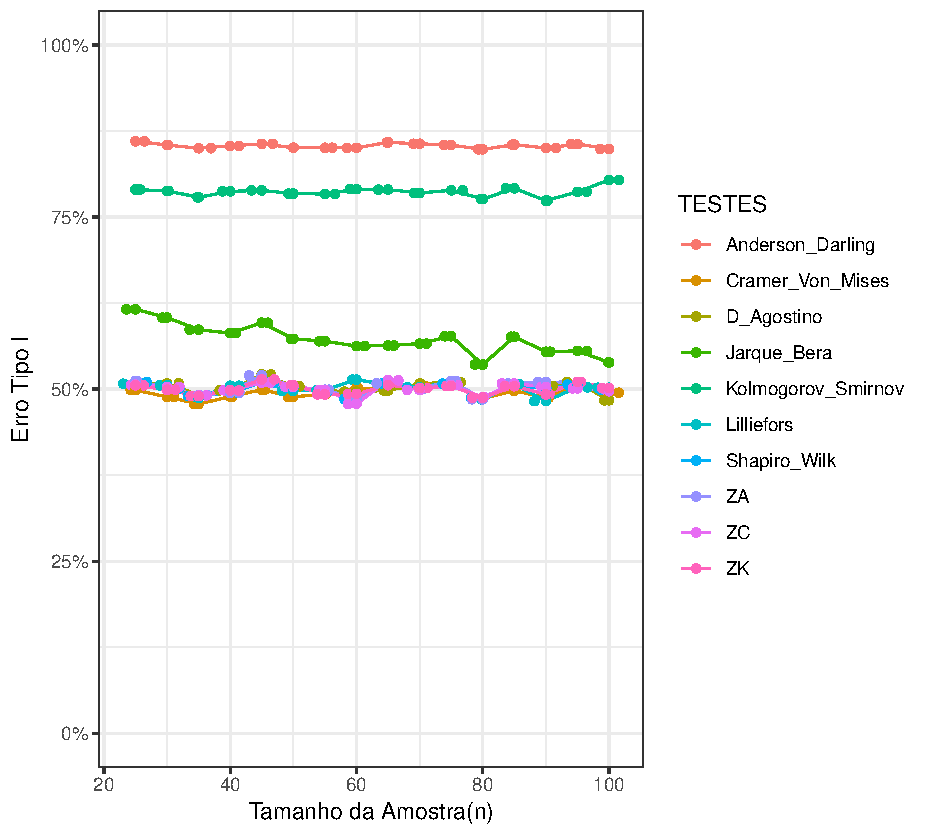
\includegraphics[width=\textwidth]{Distribuição Normal/Erro Tipo I/erro_tipo_i_normal_100.pdf}
        \caption{Tamanho amostral \(n = 100\)}
        \label{fig:normal_100}
    \end{subfigure}
    \hfill
    \begin{subfigure}[b]{0.45\textwidth}
        \centering
        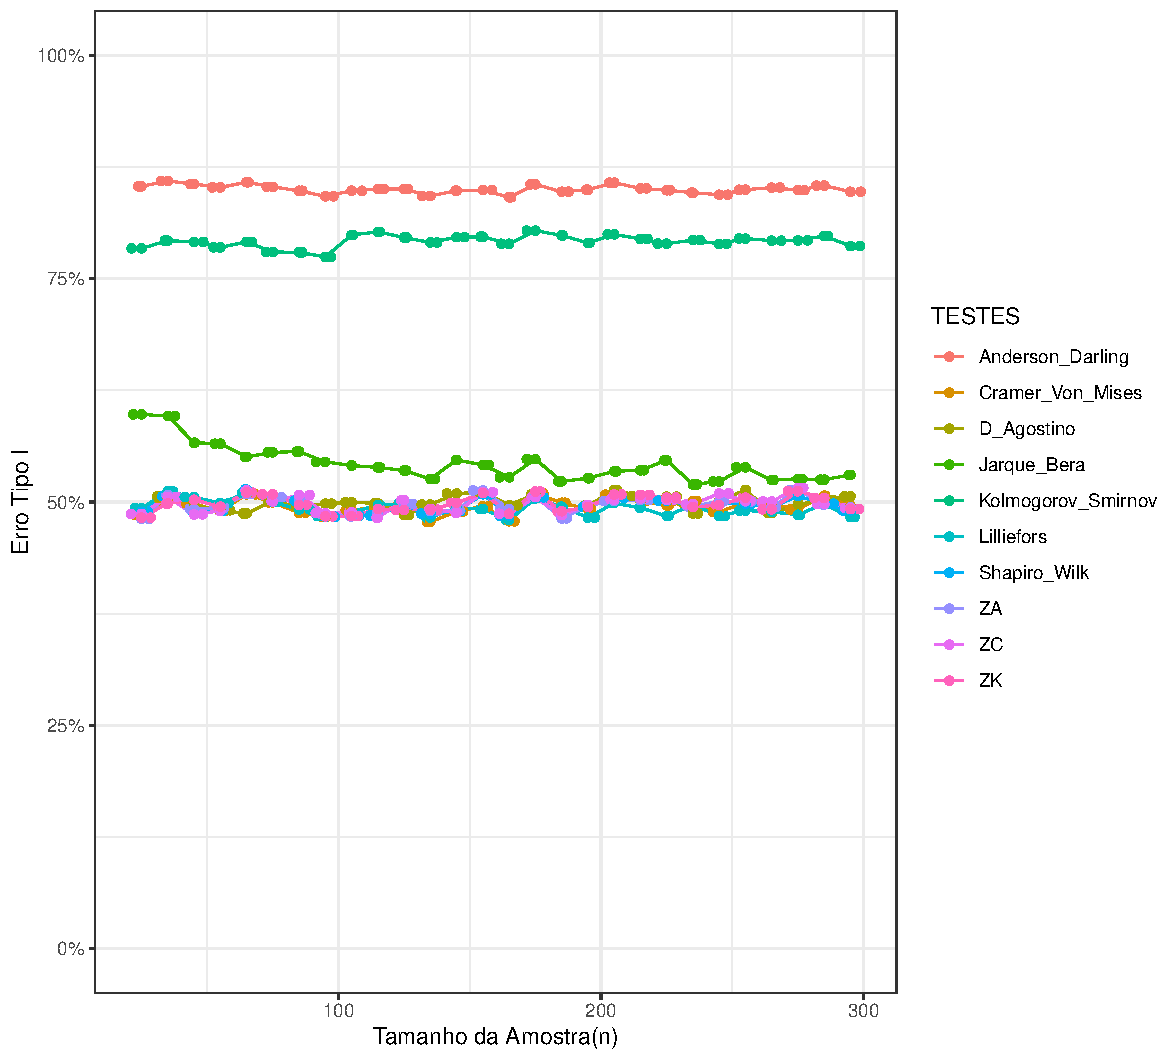
\includegraphics[width=\textwidth]{Distribuição Normal/Erro Tipo I/erro_tipo_I_normal_300.pdf}
        \caption{Tamanho amostral \(n = 300\)}
        \label{fig:normal_300}
    \end{subfigure}
    
    % Terceira linha
    \vspace{0.5cm} % Espaçamento entre linhas
    \begin{subfigure}[b]{0.45\textwidth}
        \centering
        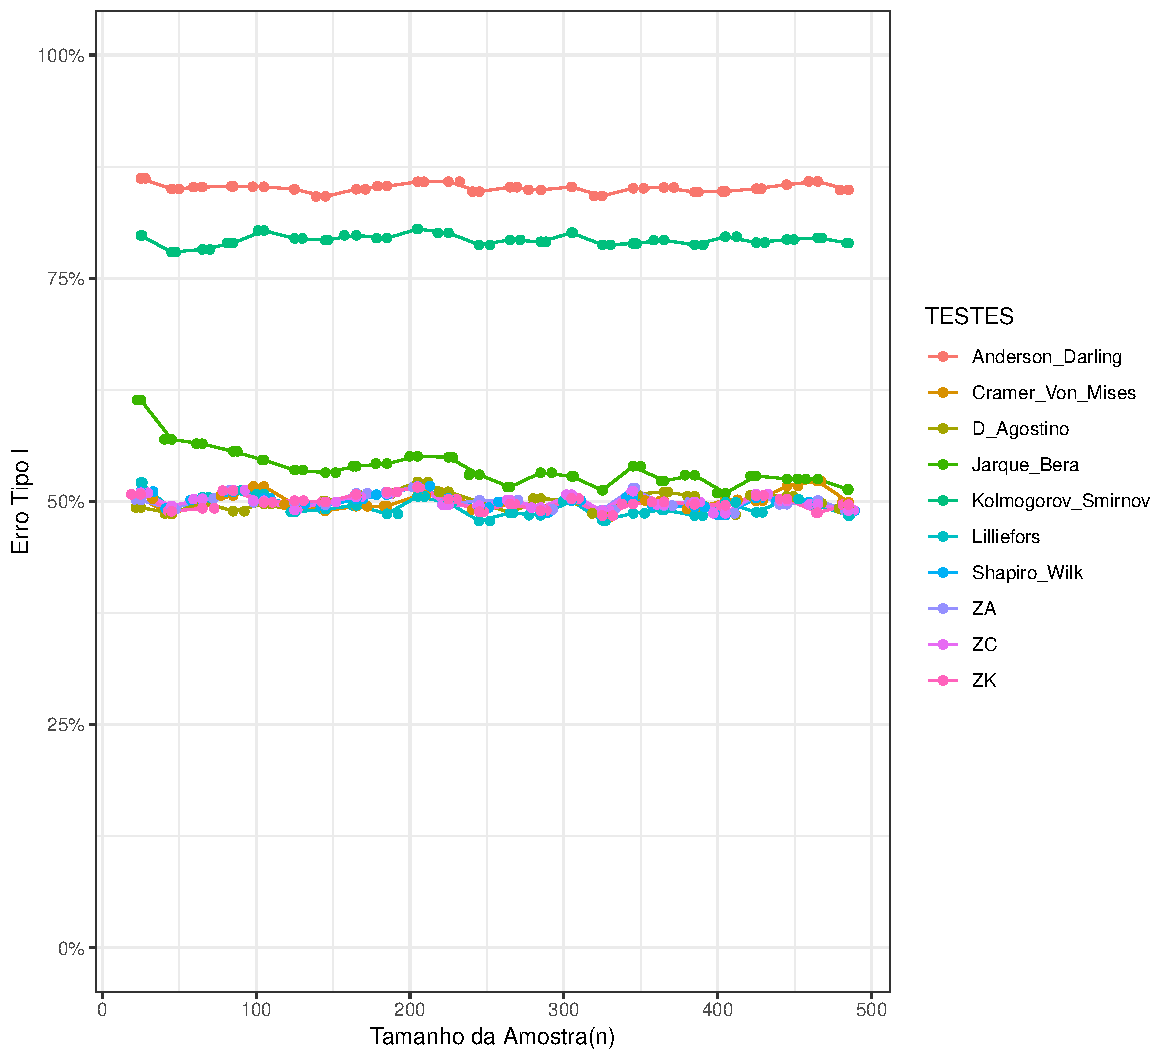
\includegraphics[width=\textwidth]{Distribuição Normal/Erro Tipo I/erro_tipo_I_normal_500.pdf}
        \caption{Tamanho amostral \(n = 500\)}
        \label{fig:normal_500}
    \end{subfigure}
    \hfill
    \begin{subfigure}[b]{0.45\textwidth}
        \centering
        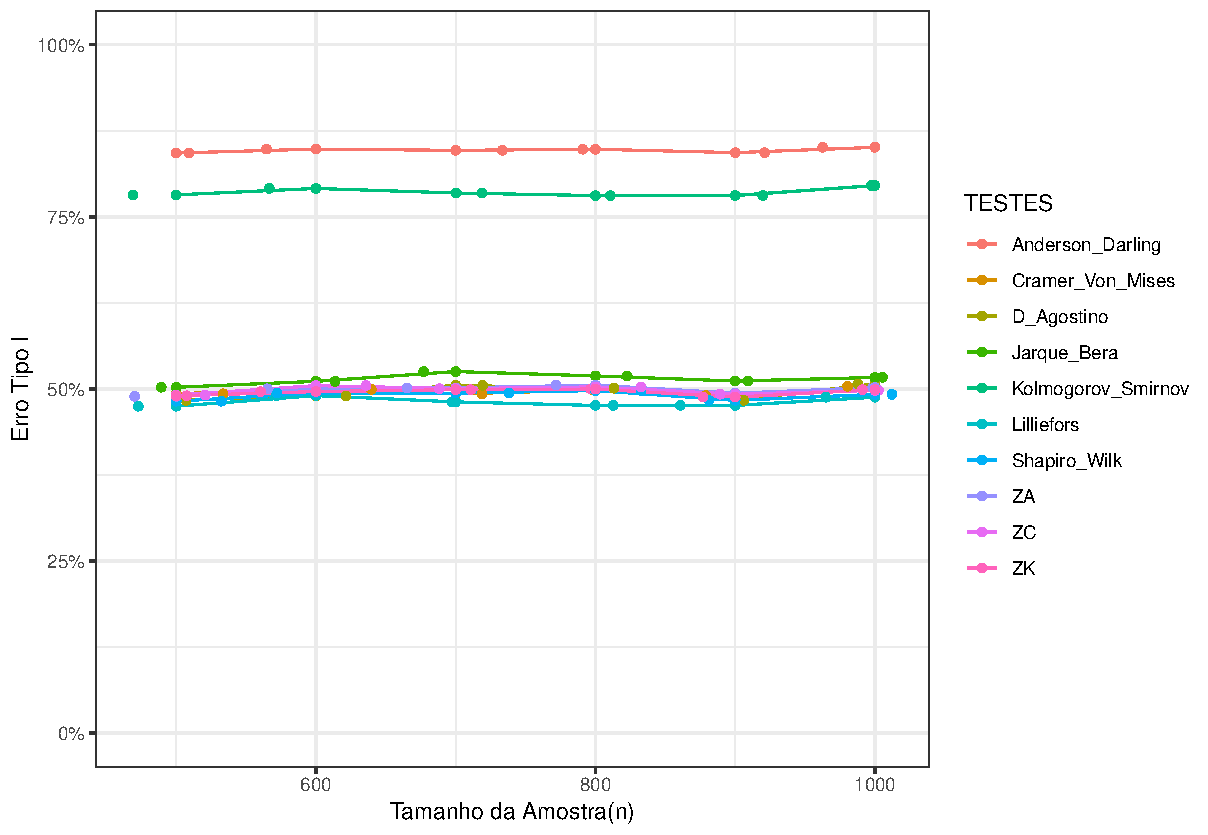
\includegraphics[width=\textwidth]{Distribuição Normal/Erro Tipo I/erro_tipo_I_normal_1000.pdf}
        \caption{Tamanho amostral \(n = 1000\)}
        \label{fig:normal_1000}
    \end{subfigure}
\end{figure}

%%%%%%%%%% Poder do Teste -> Distribuição Normal %%%%%%%%%%
\begin{figure}[H]
    \centering
    \caption{Comparação do Poder do Teste dos testes AD, CM, DG, LL, JB, KS, ZA, ZC e ZK em função do tamanho amostral para a \textbf{Distribuição} \(\textbf{Normal}(0, 1)\).}
    \label{fig:poder_teste_dist_norm}
    
    % Primeira linha
    \begin{subfigure}[b]{0.45\textwidth}
        \centering
        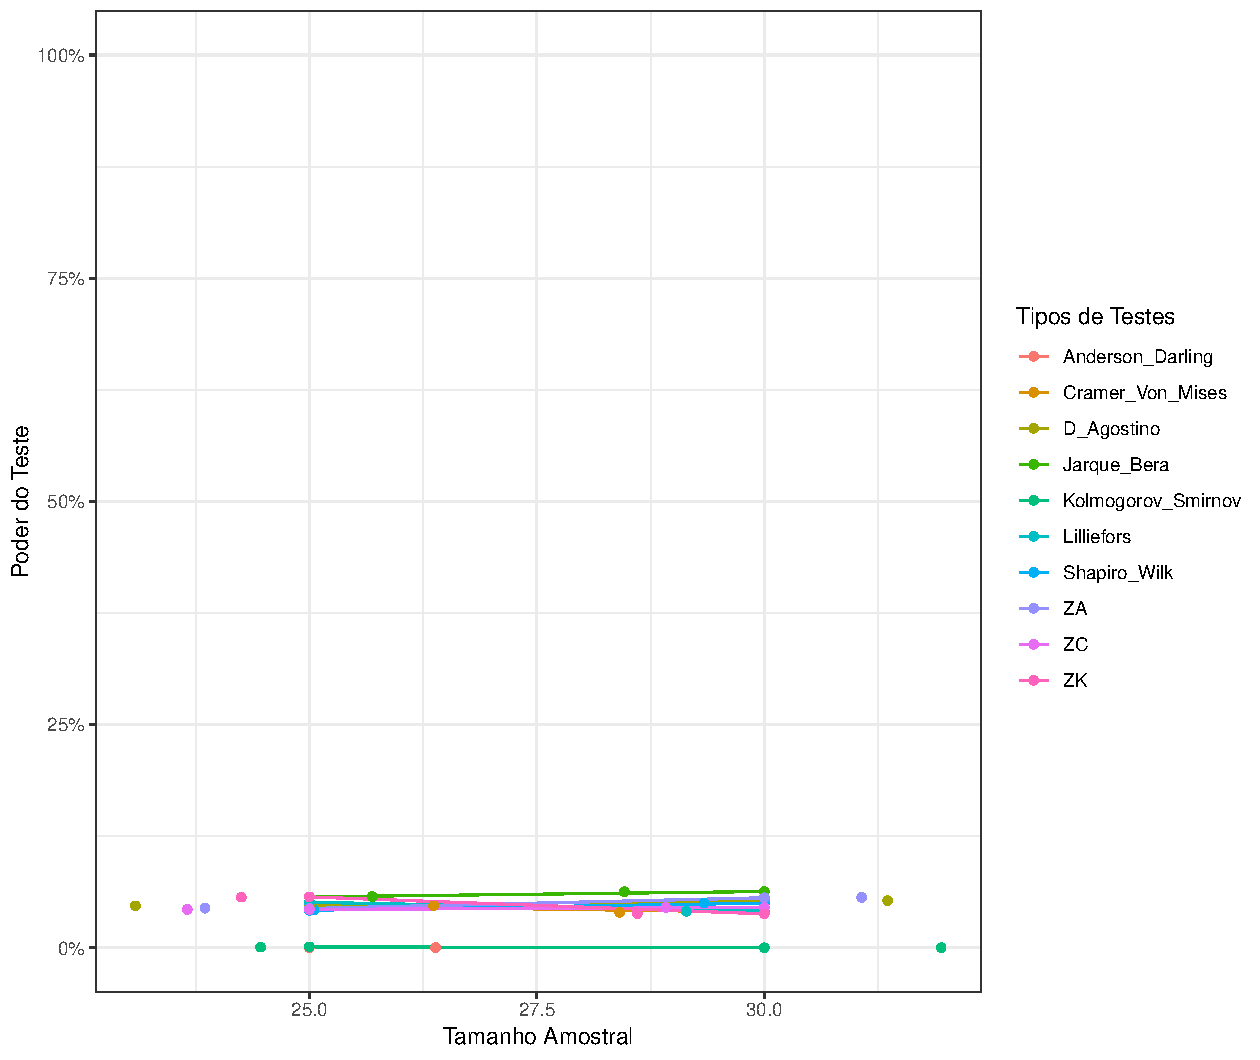
\includegraphics[width=\textwidth]{Distribuição Normal/Poder do Teste/poder_teste_normal_30.pdf}
        \caption{Tamanho amostral \(n = 30\)}
        \label{fig:normal_poder_30}
    \end{subfigure}
    \hfill
    \begin{subfigure}[b]{0.45\textwidth}
        \centering
        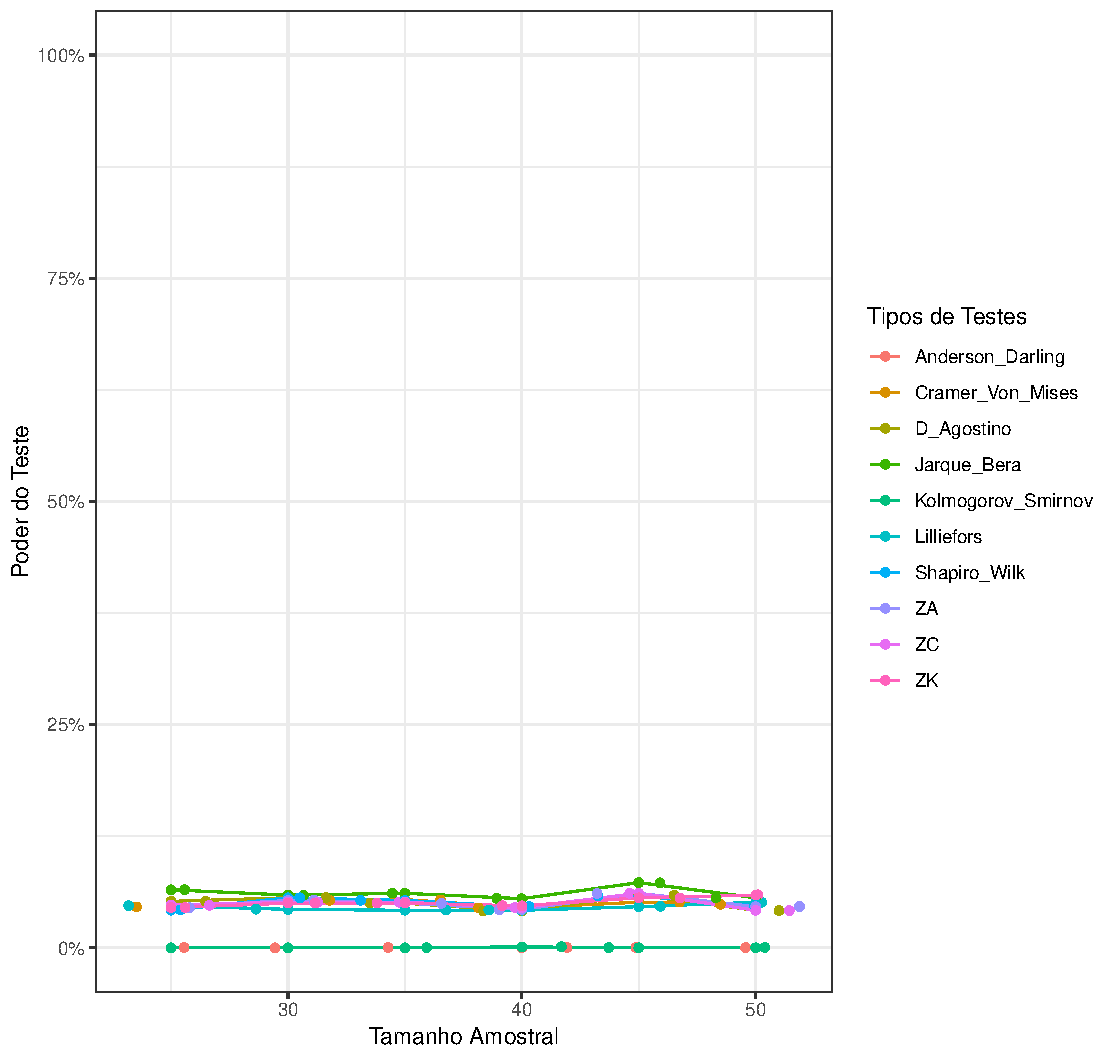
\includegraphics[width=\textwidth]{Distribuição Normal/Poder do Teste/poder_teste_normal_50.pdf}
        \caption{Tamanho amostral \(n = 50\)}
        \label{fig:normal_poder_50}
    \end{subfigure}
    
    % Segunda linha
    \vspace{0.5cm} % Espaçamento entre linhas
    \begin{subfigure}[b]{0.45\textwidth}
        \centering
        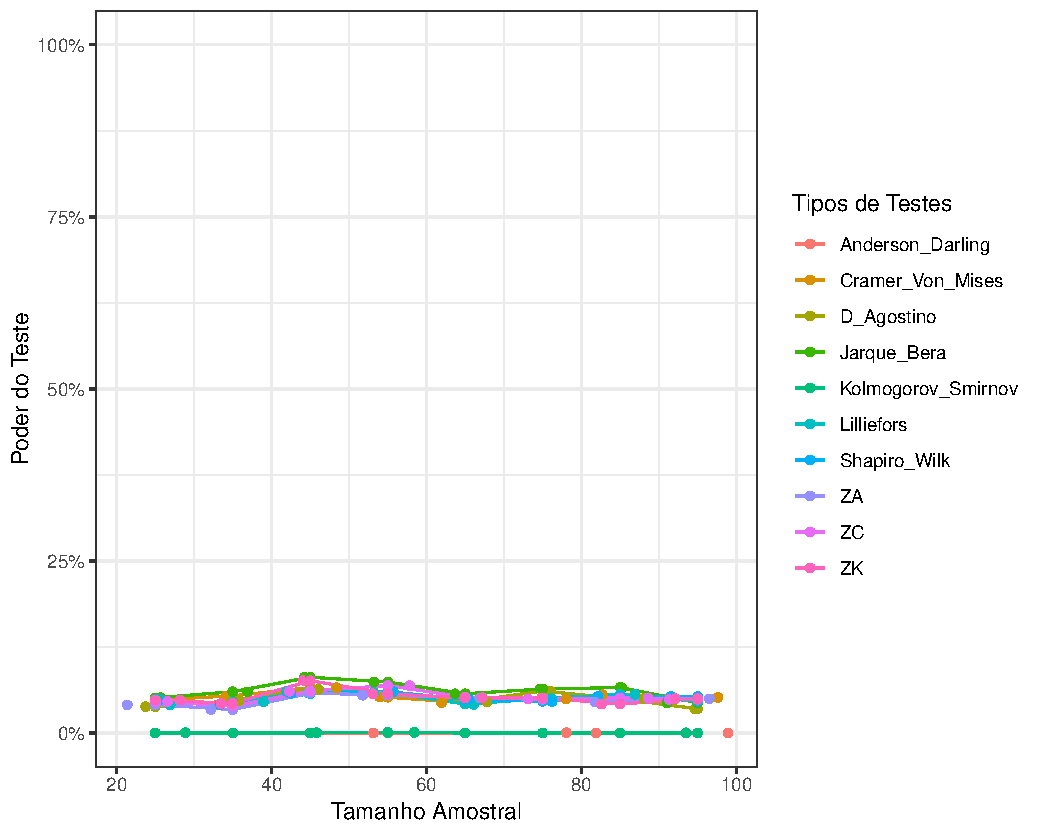
\includegraphics[width=\textwidth]{Distribuição Normal/Poder do Teste/poder_teste_normal_100.pdf}
        \caption{Tamanho amostral \(n = 100\)}
        \label{fig:normal_poder_100}
    \end{subfigure}
    \hfill
    \begin{subfigure}[b]{0.45\textwidth}
        \centering
        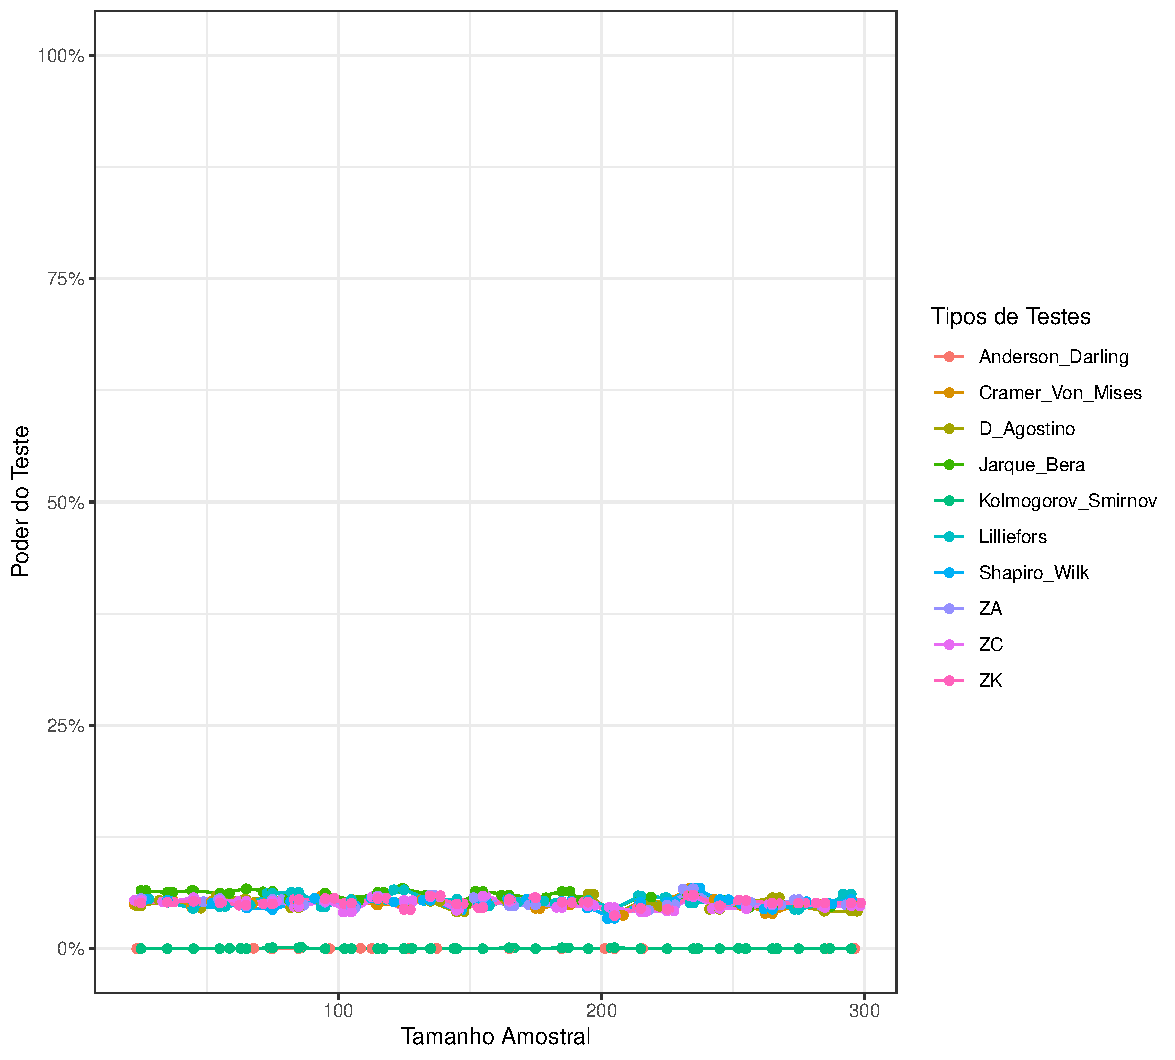
\includegraphics[width=\textwidth]{Distribuição Normal/Poder do Teste/poder_teste_normal_300.pdf}
        \caption{Tamanho amostral \(n = 300\)}
        \label{fig:normal_poder_300}
    \end{subfigure}
    
    % Terceira linha
    \vspace{0.5cm} % Espaçamento entre linhas
    \begin{subfigure}[b]{0.45\textwidth}
        \centering
        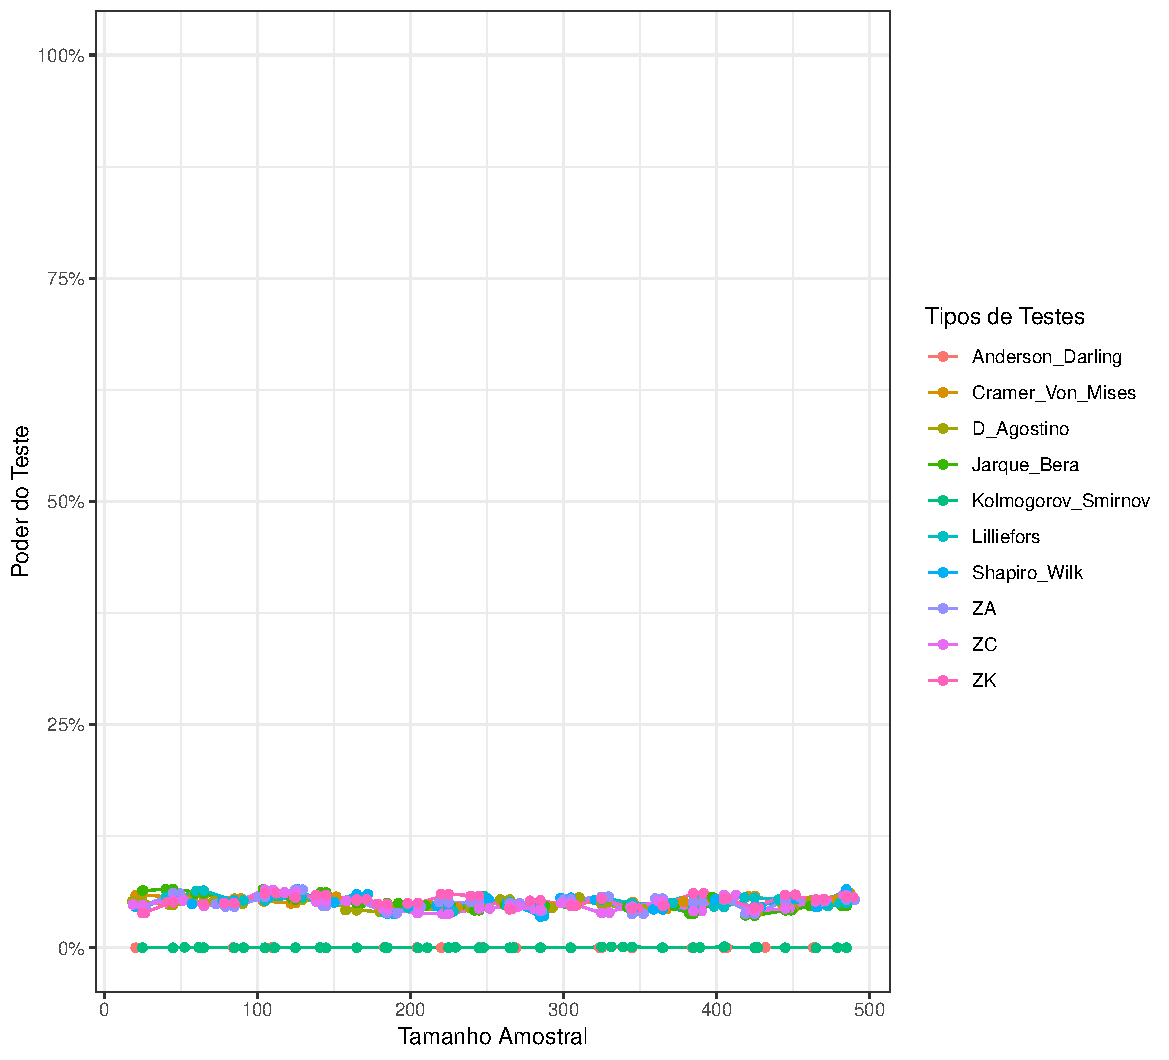
\includegraphics[width=\textwidth]{Distribuição Normal/Poder do Teste/poder_teste_normal_500.pdf}
        \caption{Tamanho amostral \(n = 500\)}
        \label{fig:normal_poder_500}
    \end{subfigure}
    \hfill
    \begin{subfigure}[b]{0.45\textwidth}
        \centering
        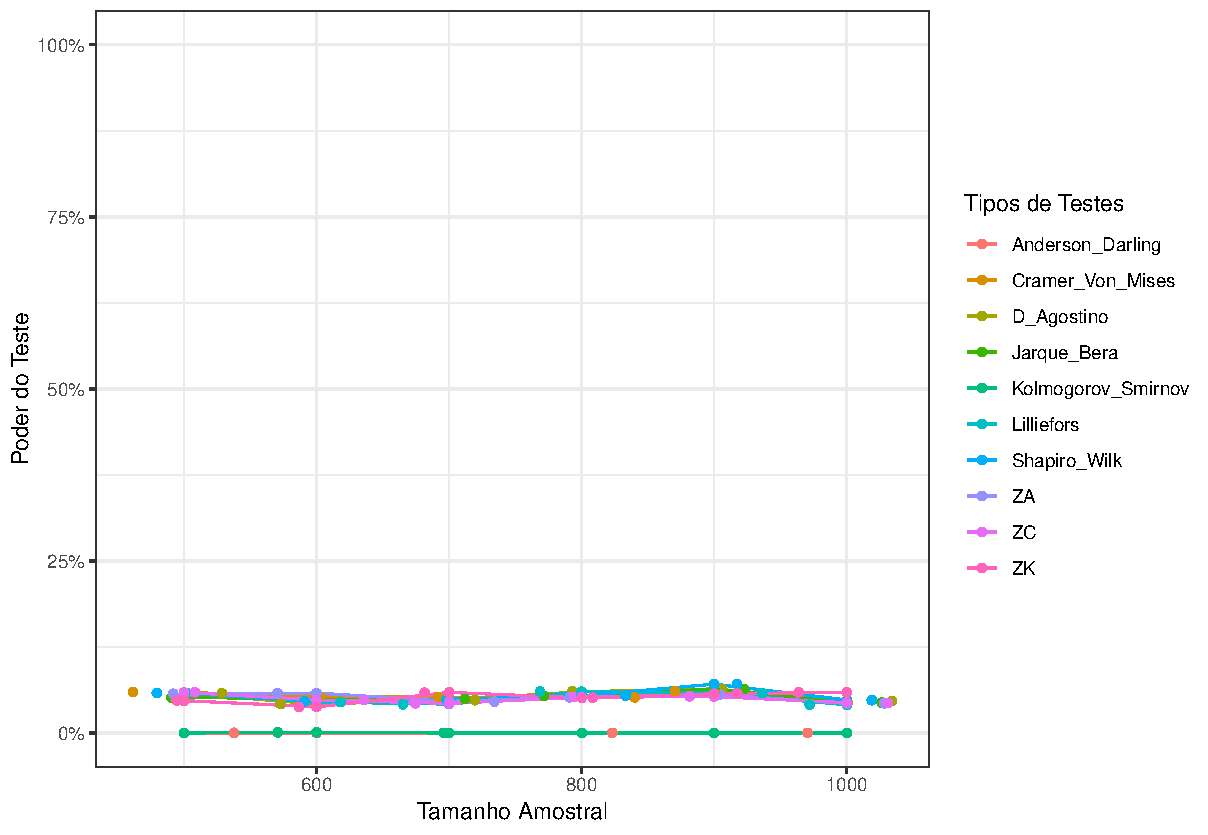
\includegraphics[width=\textwidth]{Distribuição Normal/Poder do Teste/poder_teste_normal_1000.pdf}
        \caption{Tamanho amostral \(n = 1000\)}
        \label{fig:normal_poder_1000}
    \end{subfigure}
\end{figure}

%%%%%%%%%% Erro Tipo I -> Distribuição Beta %%%%%%%%%%
\begin{figure}[H]
    \centering
    \caption{Comparação do Erro Tipo I dos testes AD, CM, DG, LL, JB, KS, LL, ZA, ZC e ZK em função do tamanho amostral para a \textbf{Distribuição} $\textbf{Beta}(2, 5)$.}
    \label{fig:erro_tipo_I_dist_beta}
    
    % Primeira linha
    \begin{subfigure}[b]{0.45\textwidth}
        \centering
        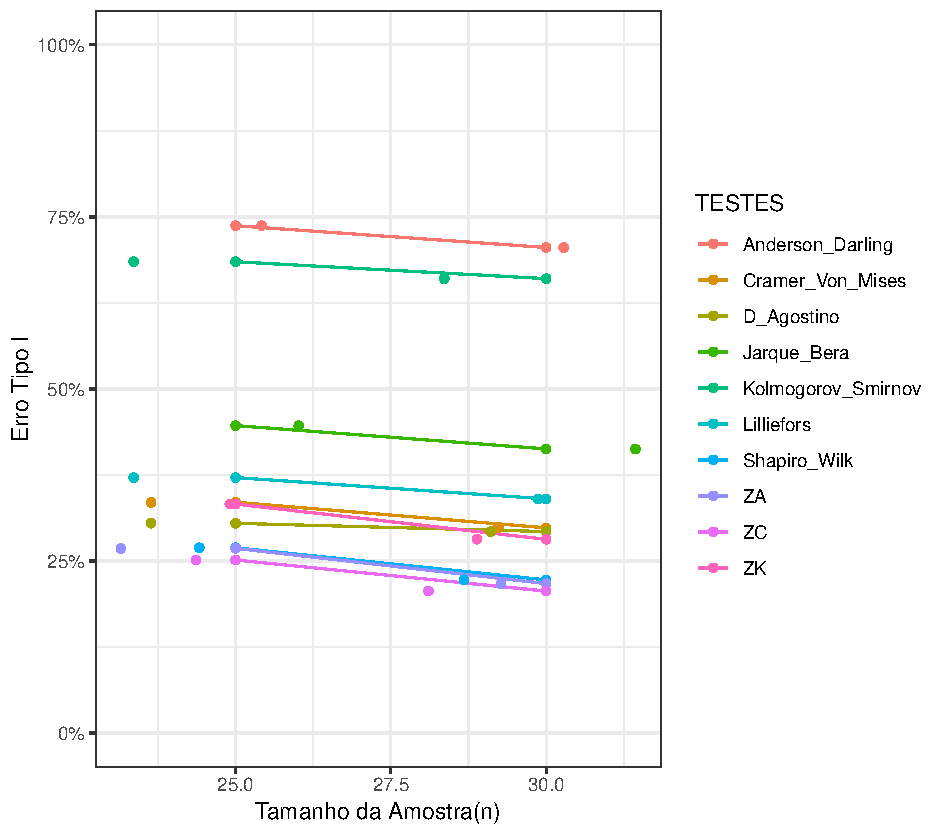
\includegraphics[width=\textwidth]{Distribuição Beta/Erro Tipo I/erro_tipo_I_beta_30.pdf}
        \caption{Tamanho amostral \(n = 30\)}
        \label{fig:beta_30}
    \end{subfigure}
    \hfill
    \begin{subfigure}[b]{0.45\textwidth}
        \centering
        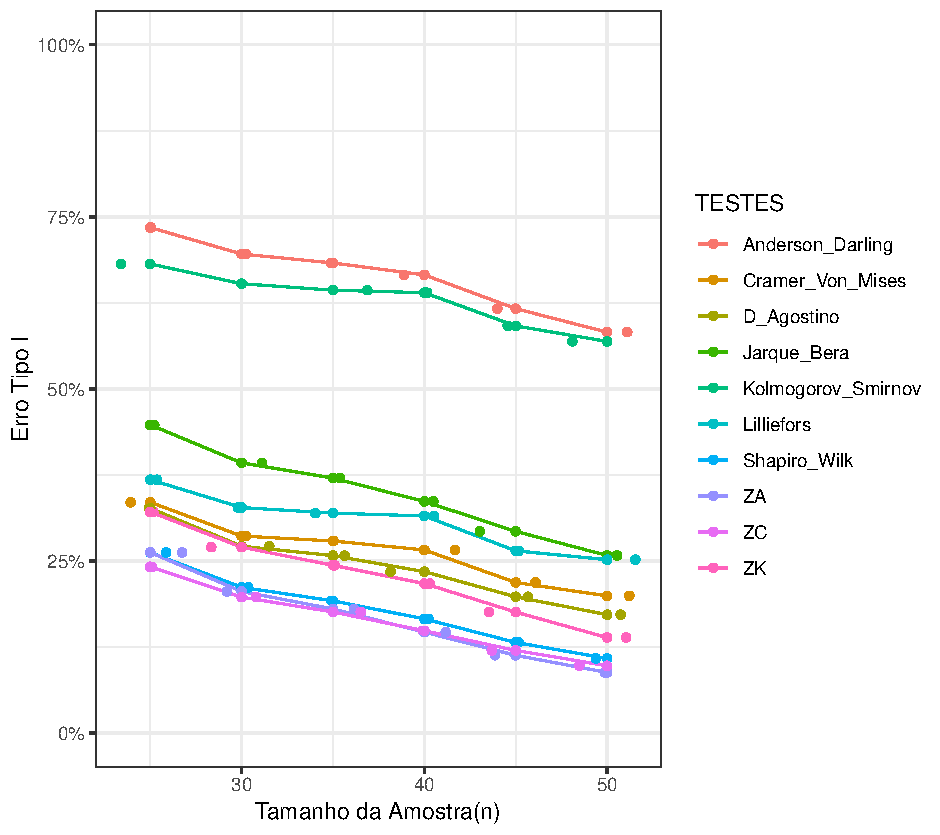
\includegraphics[width=\textwidth]{Distribuição Beta/Erro Tipo I/erro_tipo_I_beta_50.pdf}
        \caption{Tamanho amostral \(n = 50\)}
        \label{fig:beta_50}
    \end{subfigure}
    
    % Segunda linha
    \vspace{0.5cm} % Espaçamento entre linhas
    \begin{subfigure}[b]{0.45\textwidth}
        \centering
        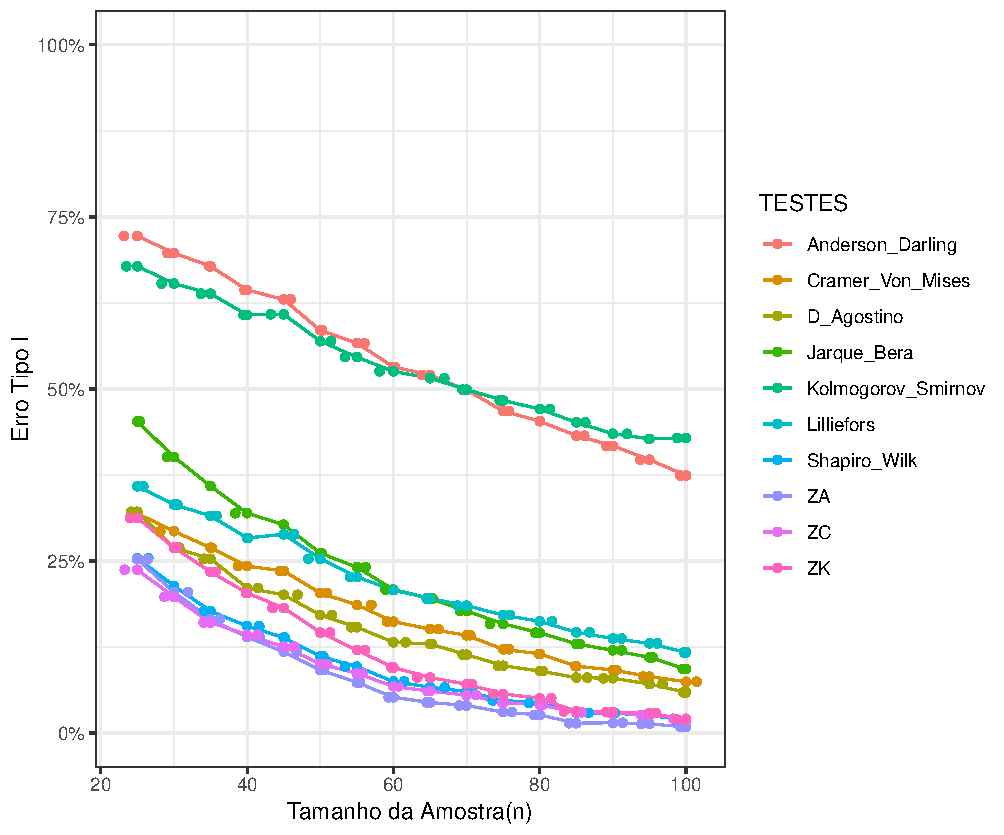
\includegraphics[width=\textwidth]{Distribuição Beta/Erro Tipo I/erro_tipo_I_beta_100.pdf}
        \caption{Tamanho amostral \(n = 100\)}
        \label{fig:beta_100}
    \end{subfigure}
    \hfill
    \begin{subfigure}[b]{0.45\textwidth}
        \centering
        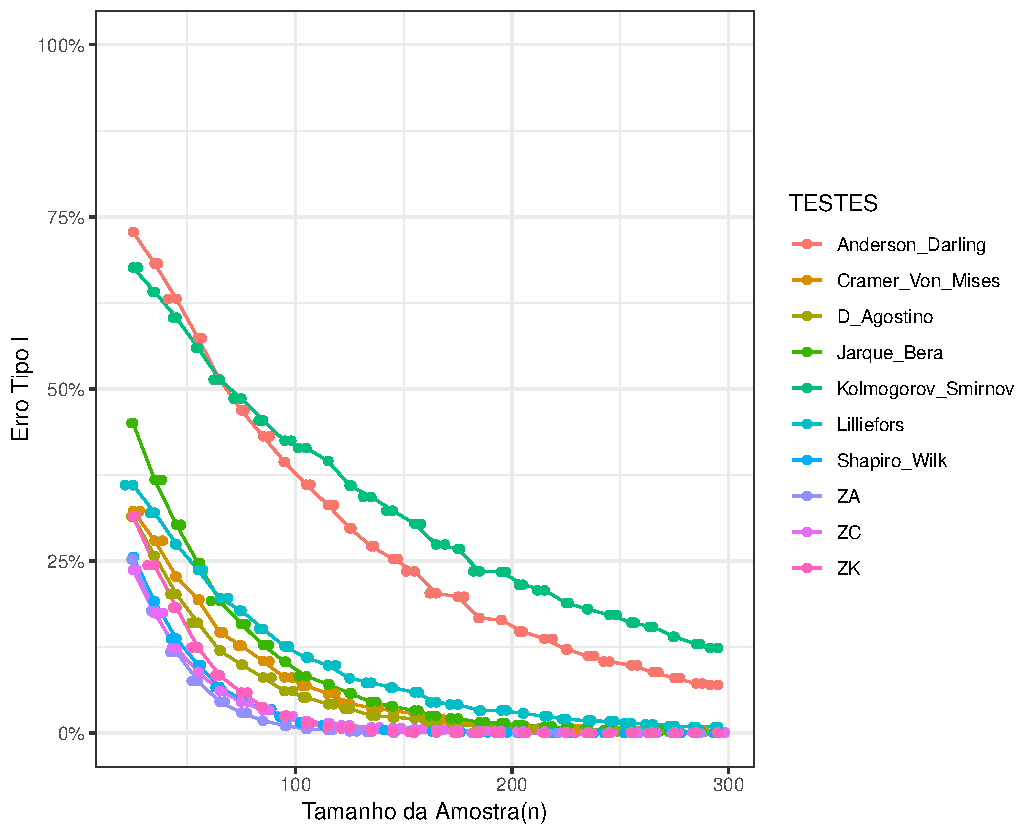
\includegraphics[width=\textwidth]{Distribuição Beta/Erro Tipo I/erro_tipo_I_beta_300.pdf}
        \caption{Tamanho amostral \(n = 300\)}
        \label{fig:beta_300}
    \end{subfigure}
    
    % Terceira linha
    \vspace{0.5cm} % Espaçamento entre linhas
    \begin{subfigure}[b]{0.45\textwidth}
        \centering
        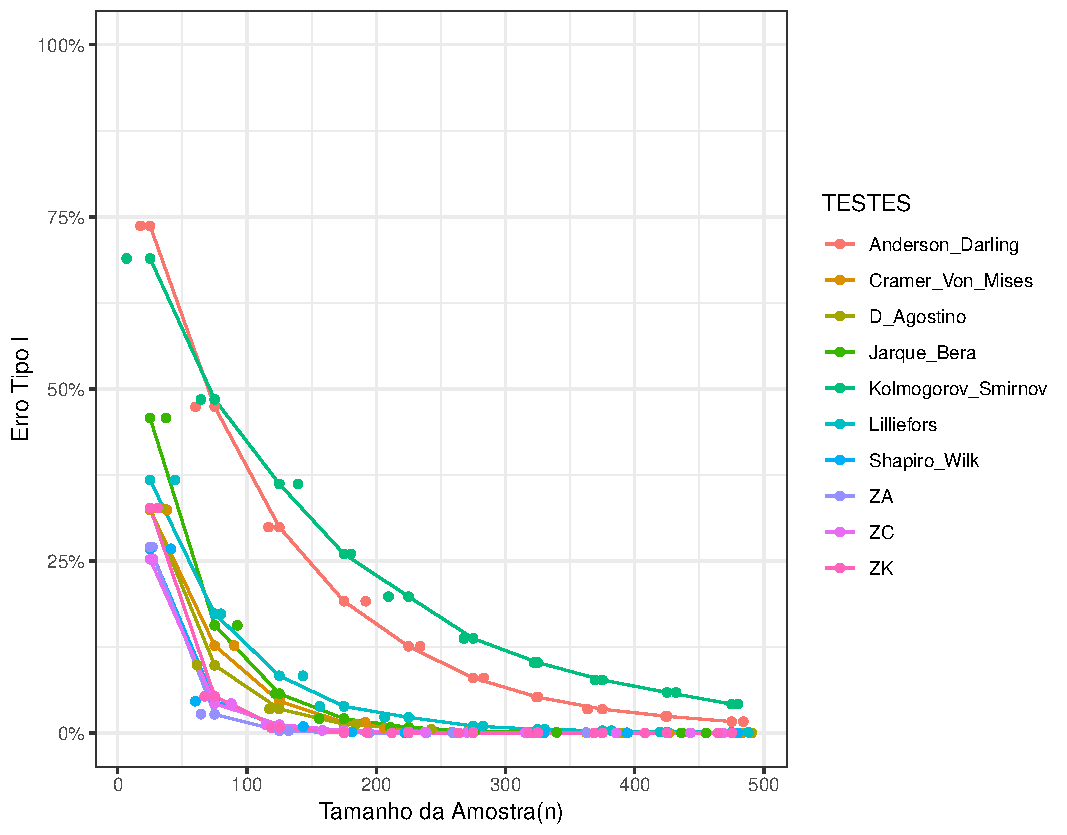
\includegraphics[width=\textwidth]{Distribuição Beta/Erro Tipo I/erro_tipo_I_beta_500.pdf}
        \caption{Tamanho amostral \(n = 500\)}
        \label{fig:beta_500}
    \end{subfigure}
    \hfill
    \begin{subfigure}[b]{0.45\textwidth}
        \centering
        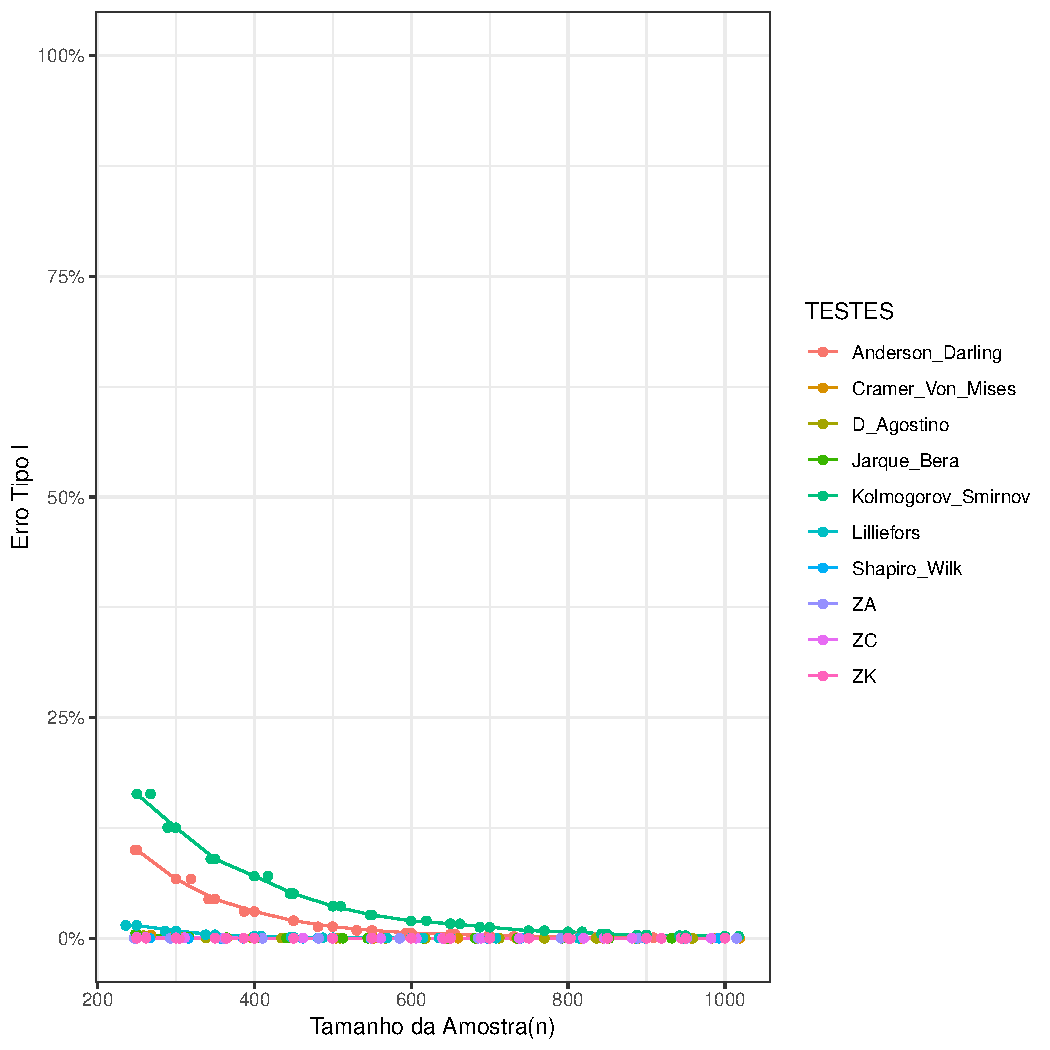
\includegraphics[width=\textwidth]{Distribuição Beta/Erro Tipo I/erro_tipo_I_beta_1000.pdf}
        \caption{Tamanho amostral \(n = 1000\)}
        \label{fig:beta_1000}
    \end{subfigure}
\end{figure}

%%%%%%%%%% Poder do Teste -> Distribuição Beta %%%%%%%%%%
\begin{figure}[H]
    \centering
    \caption{Comparação do Poder do Teste dos testes AD, CM, DG, LL, JB, KS, ZA, ZC e ZK em função do tamanho amostral para a \textbf{Distribuição} \(\textbf{Beta}(2, 5)\).}
    \label{fig:poder_teste_dist_beta}
    
    % Primeira linha
    \begin{subfigure}[b]{0.45\textwidth}
        \centering
        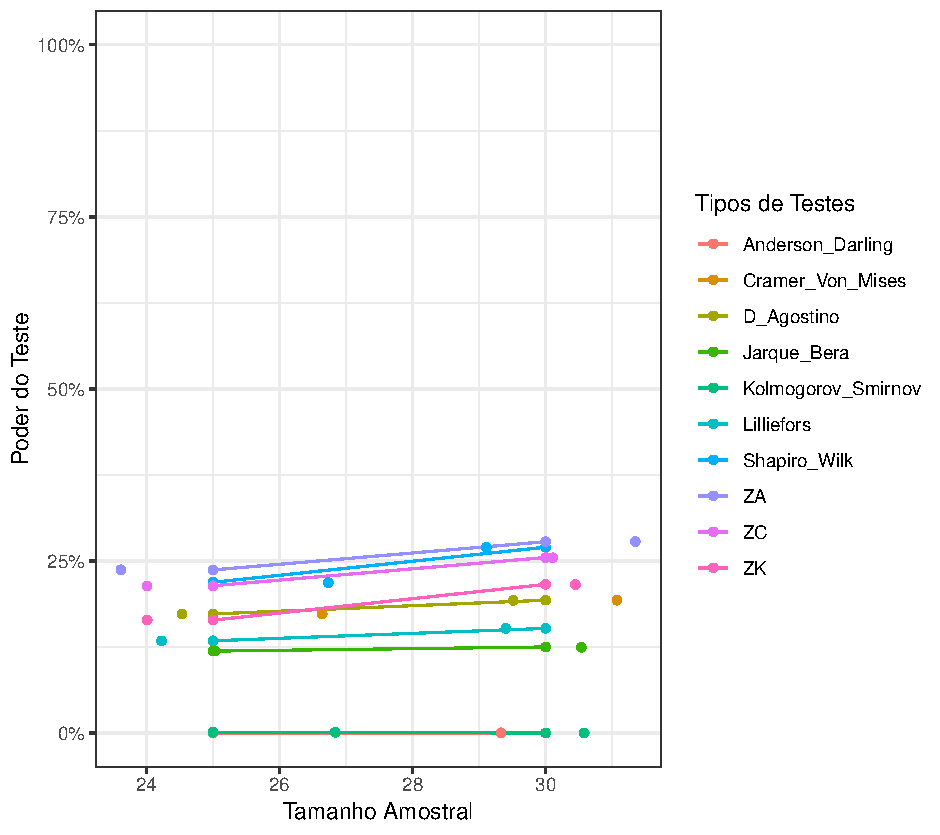
\includegraphics[width=\textwidth]{Distribuição Beta/Poder do Teste/poder_teste_beta_30.pdf}
        \caption{Tamanho amostral \(n = 30\)}
        \label{fig:beta_poder_30}
    \end{subfigure}
    \hfill
    \begin{subfigure}[b]{0.45\textwidth}
        \centering
        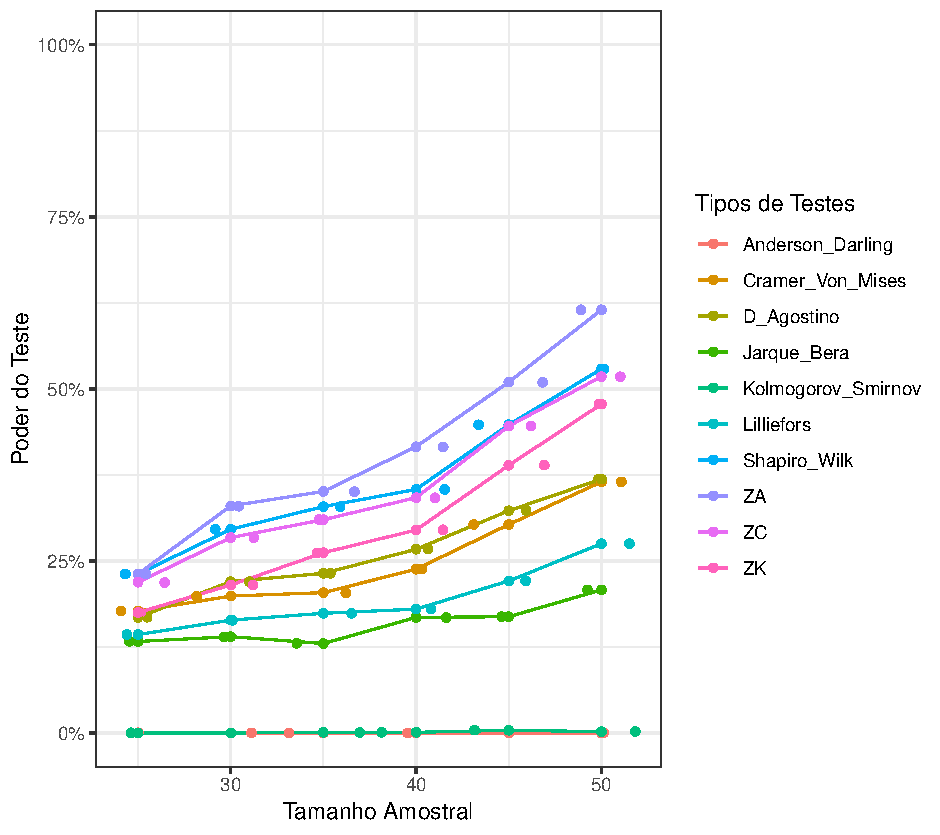
\includegraphics[width=\textwidth]{Distribuição Beta/Poder do Teste/poder_teste_beta_50.pdf}
        \caption{Tamanho amostral \(n = 50\)}
        \label{fig:beta_poder_50}
    \end{subfigure}
    
    % Segunda linha
    \vspace{0.5cm} % Espaçamento entre linhas
    \begin{subfigure}[b]{0.45\textwidth}
        \centering
        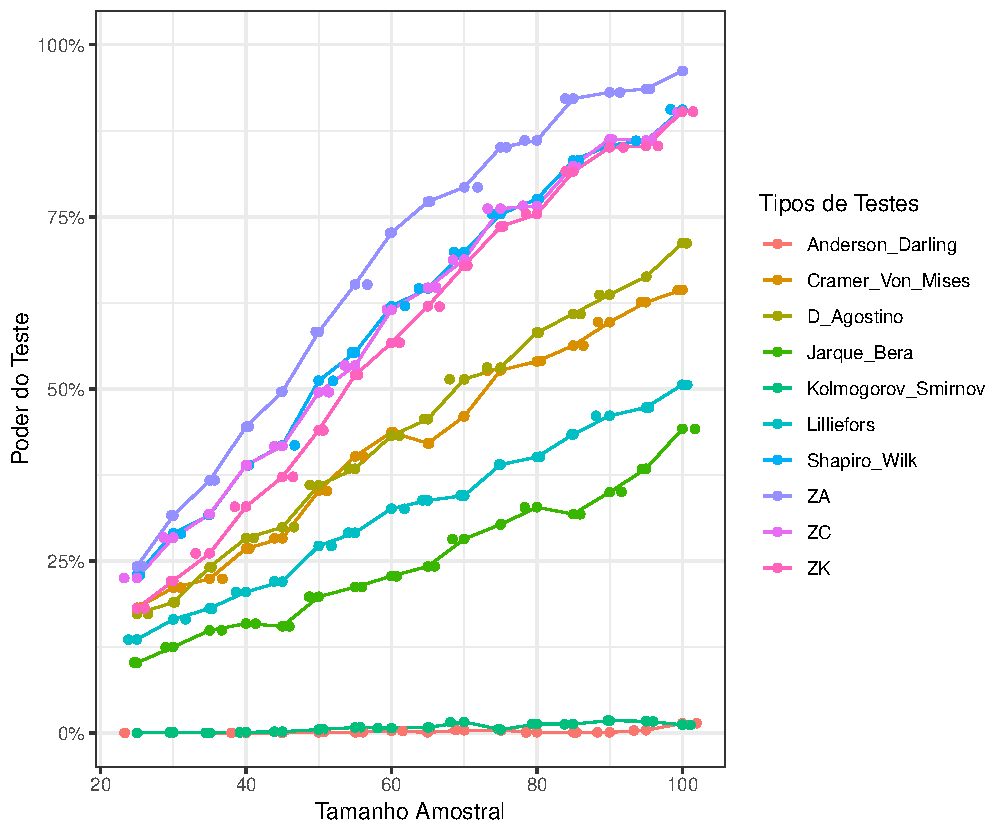
\includegraphics[width=\textwidth]{Distribuição Beta/Poder do Teste/poder_teste_beta_100.pdf}
        \caption{Tamanho amostral \(n = 100\)}
        \label{fig:beta_poder_100}
    \end{subfigure}
    \hfill
    \begin{subfigure}[b]{0.45\textwidth}
        \centering
        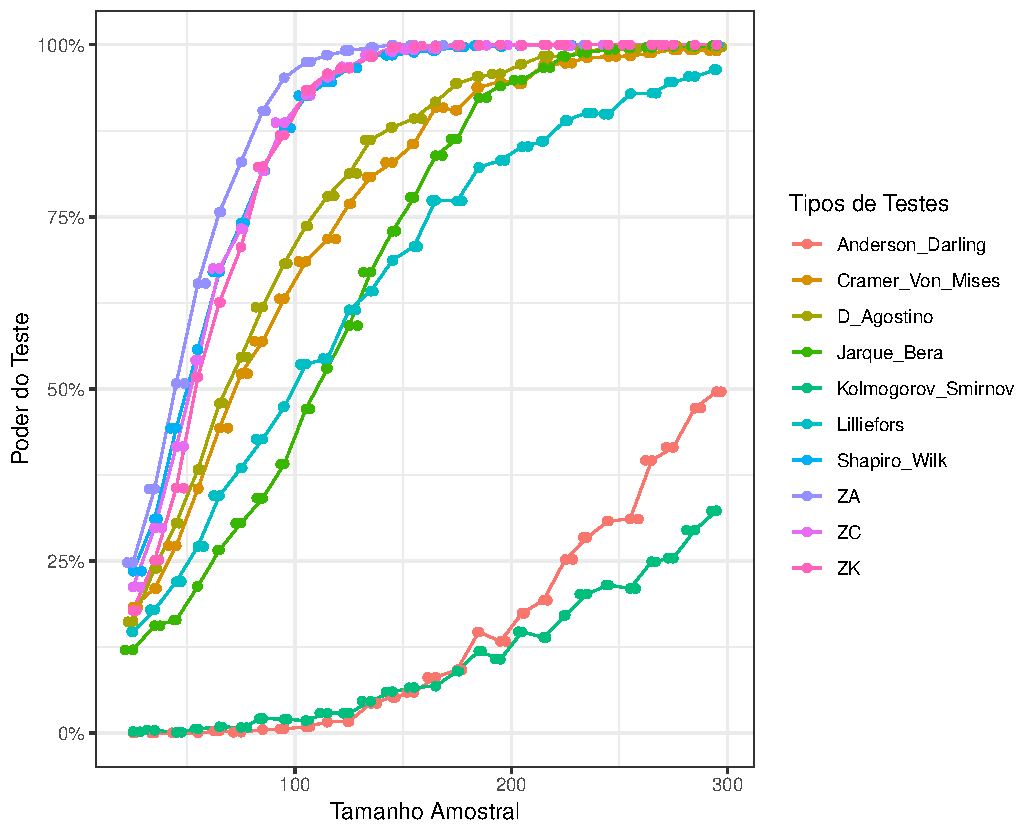
\includegraphics[width=\textwidth]{Distribuição Beta/Poder do Teste/poder_teste_beta_300.pdf}
        \caption{Tamanho amostral \(n = 300\)}
        \label{fig:beta_poder_300}
    \end{subfigure}
    
    % Terceira linha
    \vspace{0.5cm} % Espaçamento entre linhas
    \begin{subfigure}[b]{0.45\textwidth}
        \centering
        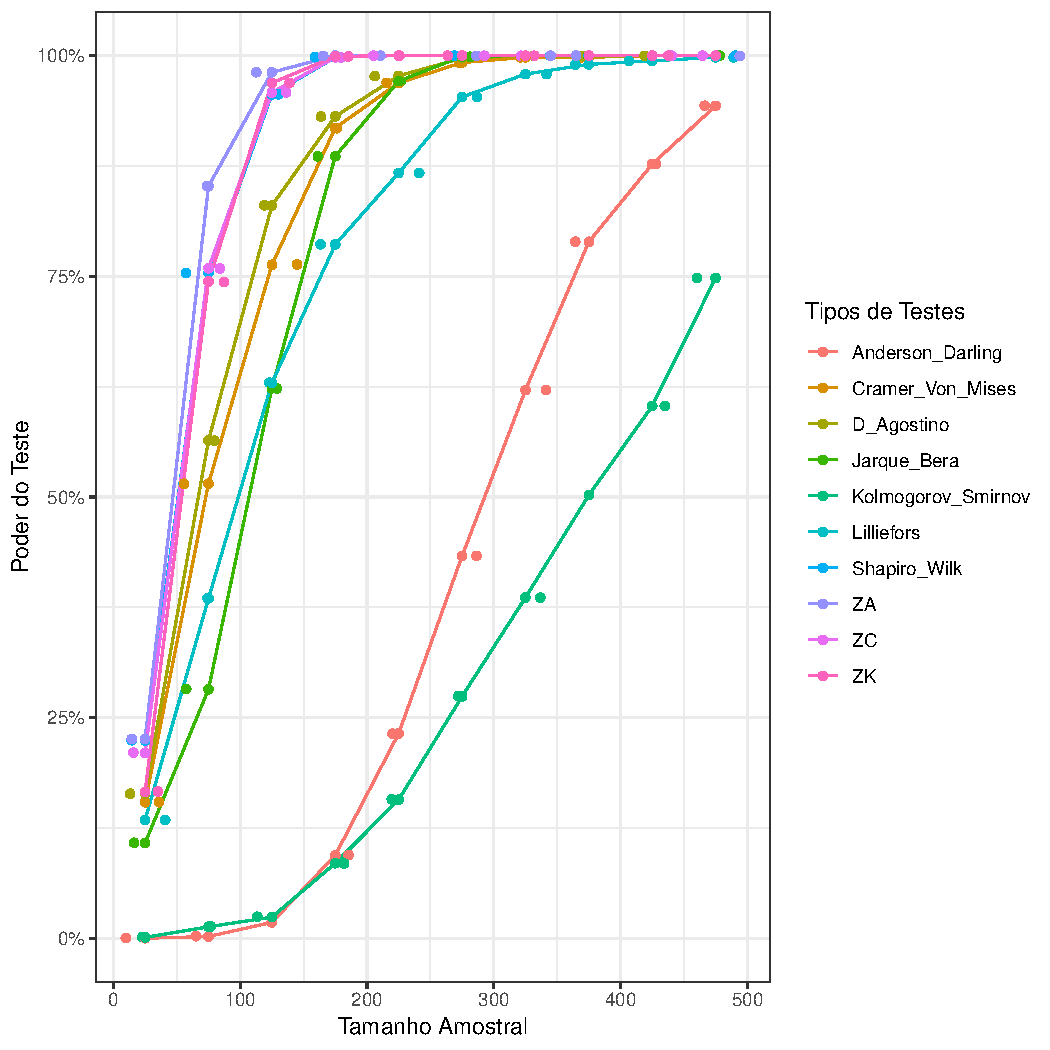
\includegraphics[width=\textwidth]{Distribuição Beta/Poder do Teste/poder_teste_beta_500.pdf}
        \caption{Tamanho amostral \(n = 500\)}
        \label{fig:beta_poder_500}
    \end{subfigure}
    \hfill
    \begin{subfigure}[b]{0.45\textwidth}
        \centering
        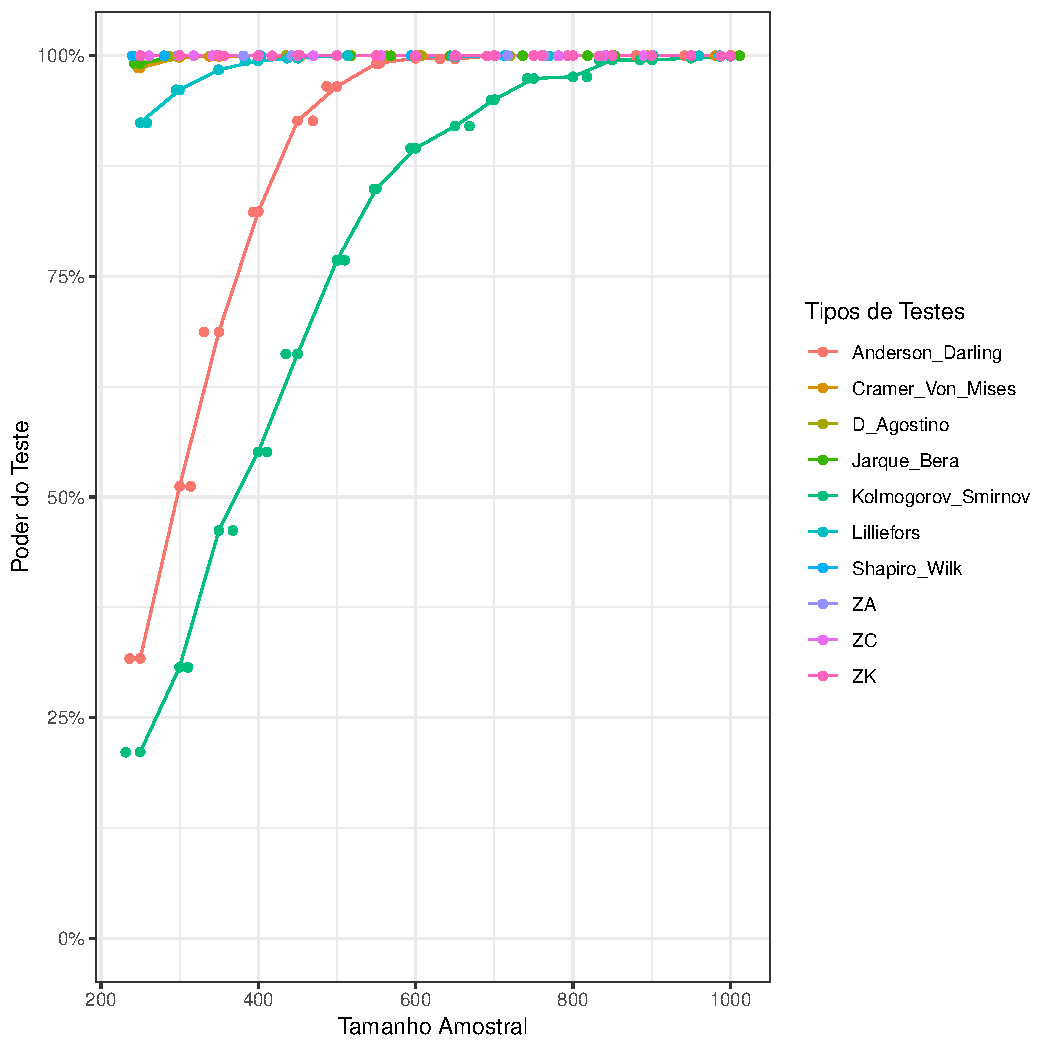
\includegraphics[width=\textwidth]{Distribuição Beta/Poder do Teste/poder_teste_beta_1000.pdf}
        \caption{Tamanho amostral \(n = 1000\)}
        \label{fig:beta_poder_1000}
    \end{subfigure}
\end{figure}


%%%%%%%%%%%%%%%%%%%%%%%%%%%%%%%%%%%%%%%%%%%%%%%%%%%%%%%%%%%%%%%%%%%%%%%%%%%%%%%%%%%%%%%%%%%%

%%%%%%%%%% Erro Tipo I -> Distribuição Cauchy %%%%%%%%%%
\begin{figure}[H]
    \centering
    \caption{Comparação do Erro Tipo I dos testes AD, CM, DG, LL, JB, KS, LL, ZA, ZC e ZK em função do tamanho amostral para a \textbf{Distribuição} $\textbf{Cauchy}(0, 1)$.}
    \label{fig:erro_tipo_I_dist_cauchy}
    
    % Primeira linha
    \begin{subfigure}[b]{0.45\textwidth}
        \centering
    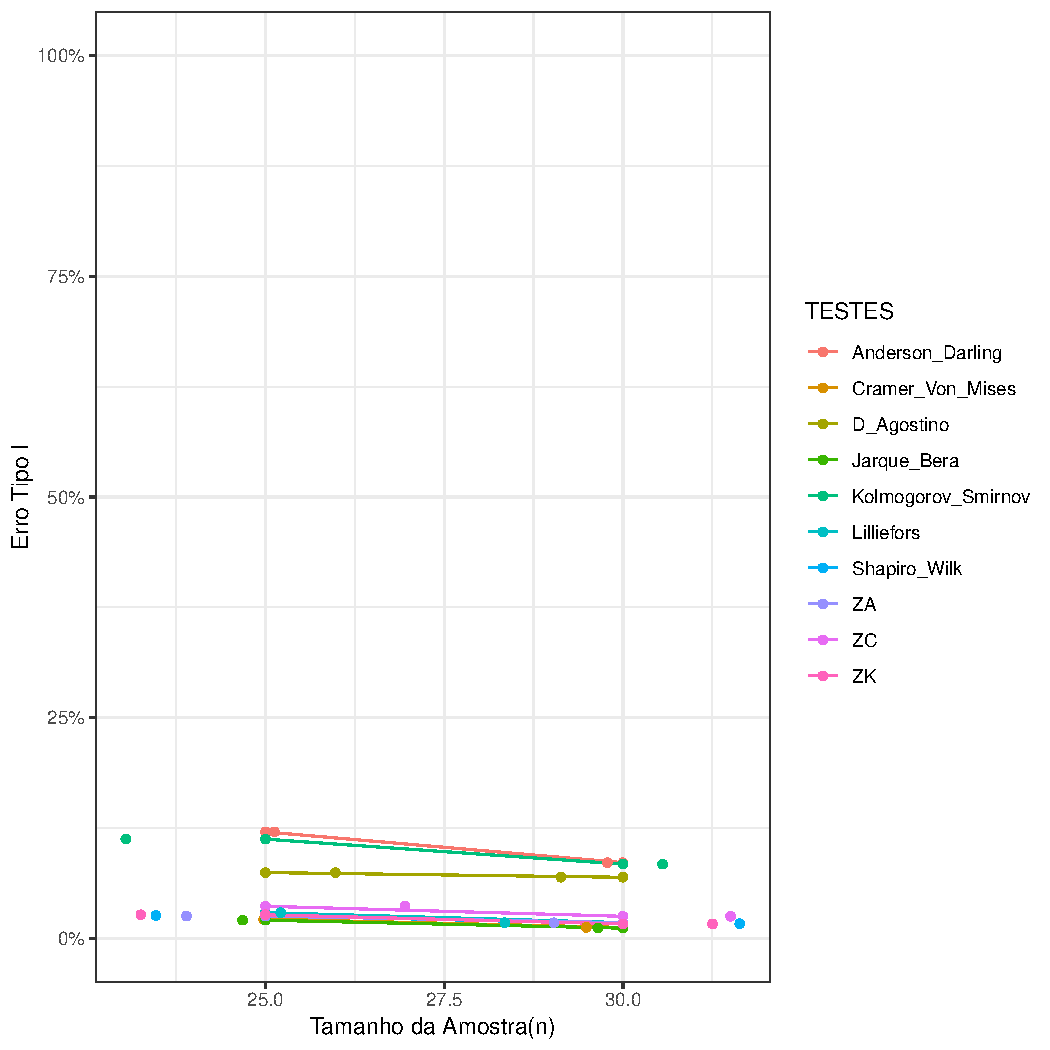
\includegraphics[width=\textwidth]{Distribuição Cauchy/Erro Tipo I/erro_tipo_I_cauchy_30.pdf}
        \caption{Tamanho amostral \(n = 30\)}
        \label{fig:cauchy_30}
    \end{subfigure}
    \hfill
    \begin{subfigure}[b]{0.45\textwidth}
        \centering
        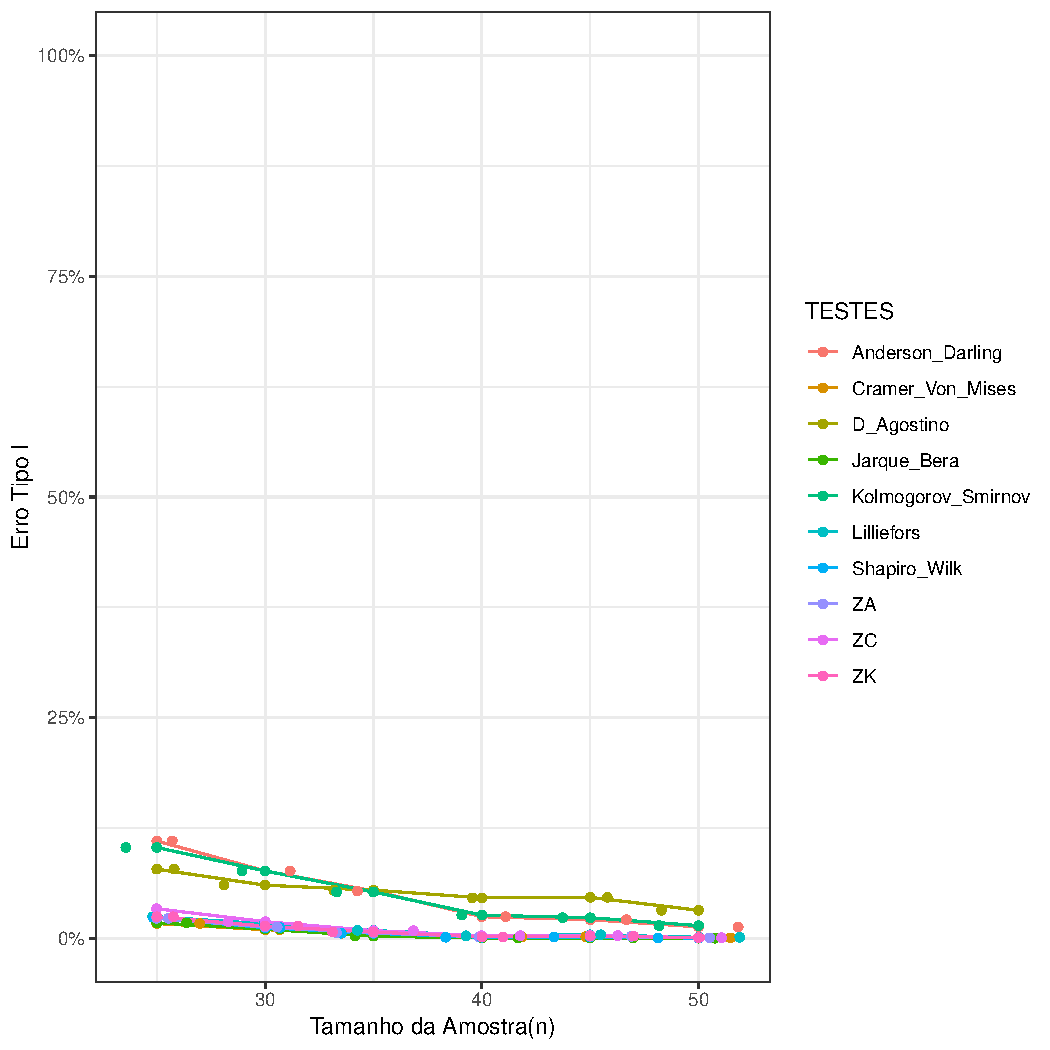
\includegraphics[width=\textwidth]{Distribuição Cauchy/Erro Tipo I/erro_tipo_I_cauchy_50.pdf}
        \caption{Tamanho amostral \(n = 50\)}
        \label{fig:cauchy_50}
    \end{subfigure}
    
    % Segunda linha
    \vspace{0.5cm} % Espaçamento entre linhas
    \begin{subfigure}[b]{0.45\textwidth}
        \centering
        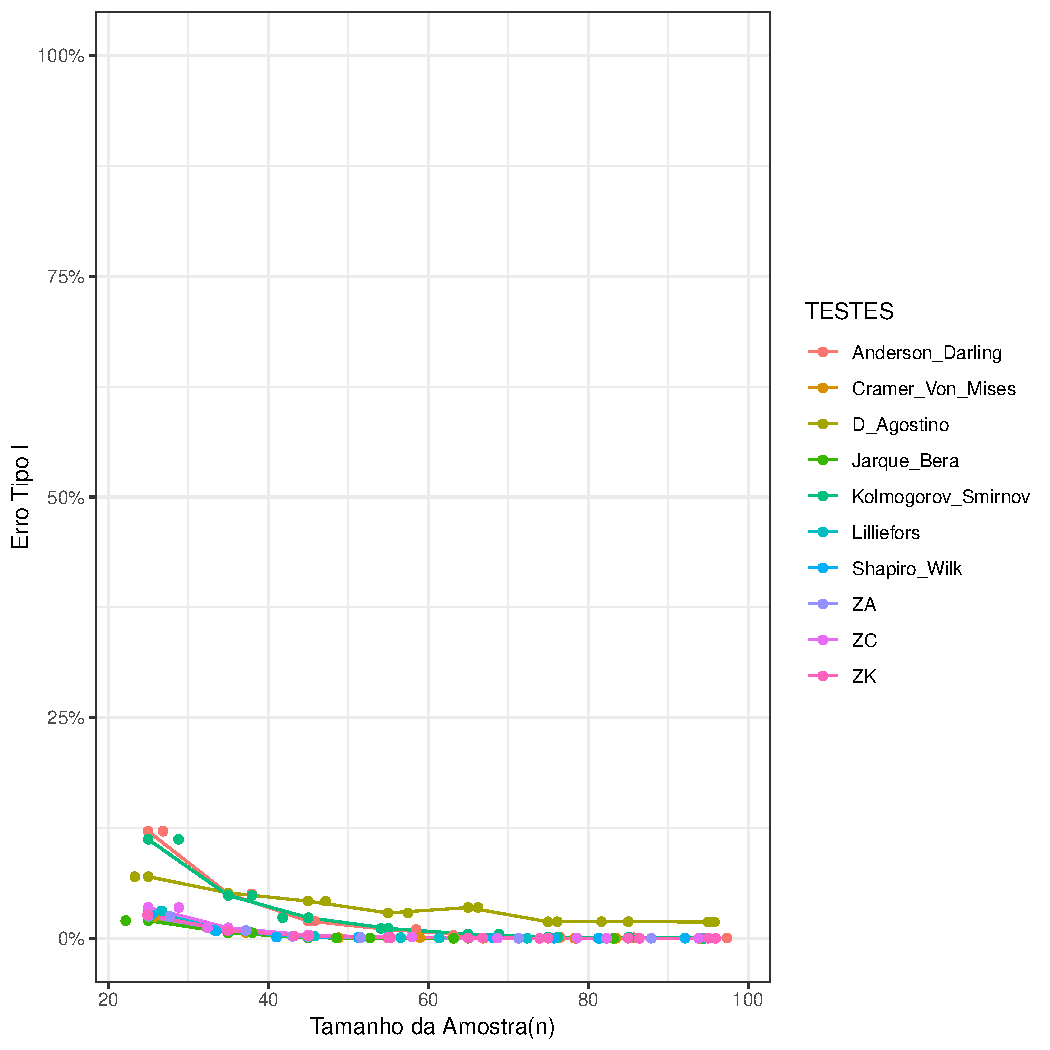
\includegraphics[width=\textwidth]{Distribuição Cauchy/Erro Tipo I/erro_tipo_I_cauchy_100.pdf}
        \caption{Tamanho amostral \(n = 100\)}
        \label{fig:cauchy_100}
    \end{subfigure}
    \hfill
    \begin{subfigure}[b]{0.45\textwidth}
        \centering
        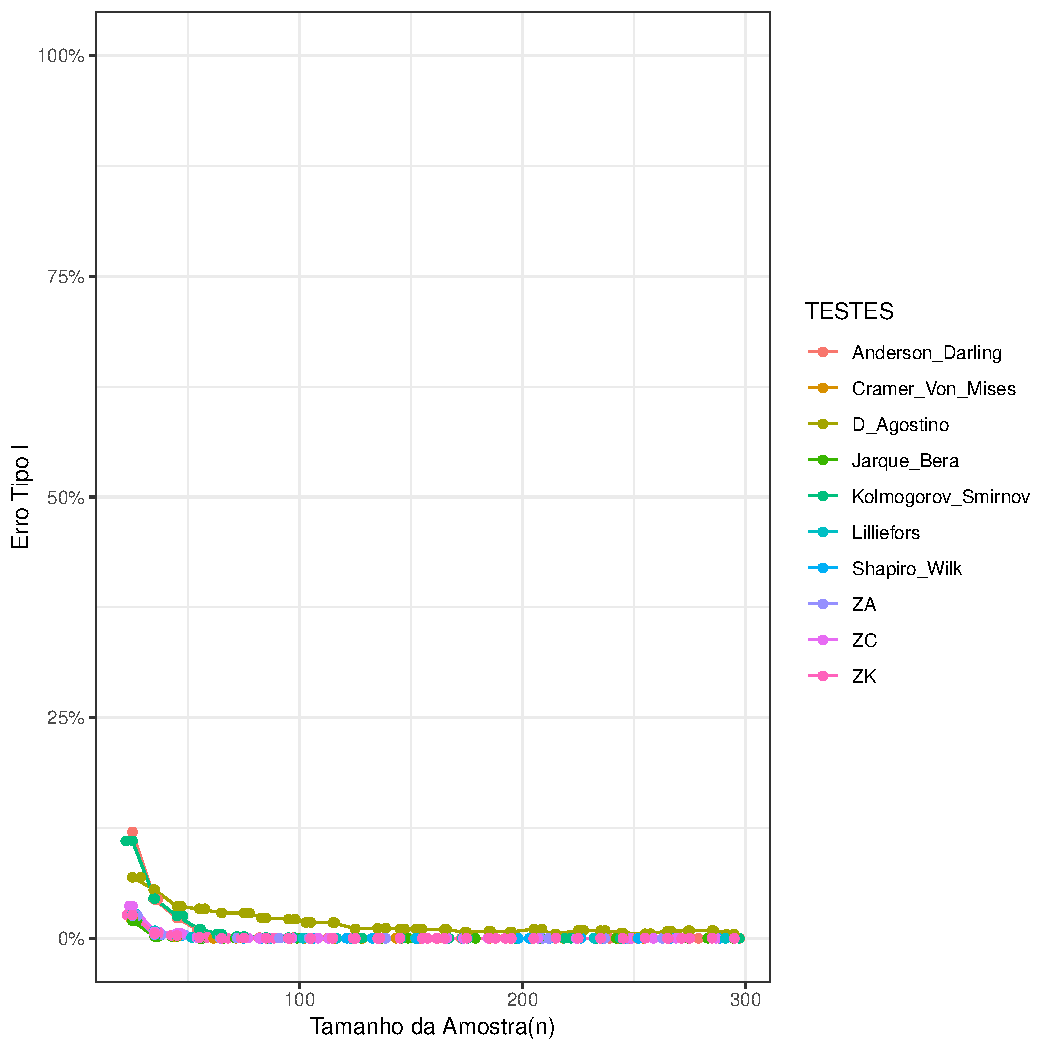
\includegraphics[width=\textwidth]{Distribuição cauchy/Erro Tipo I/erro_tipo_I_cauchy_300.pdf}
        \caption{Tamanho amostral \(n = 300\)}
        \label{fig:cauchy_300}
    \end{subfigure}
    
    % Terceira linha
    \vspace{0.5cm} % Espaçamento entre linhas
    \begin{subfigure}[b]{0.45\textwidth}
        \centering
        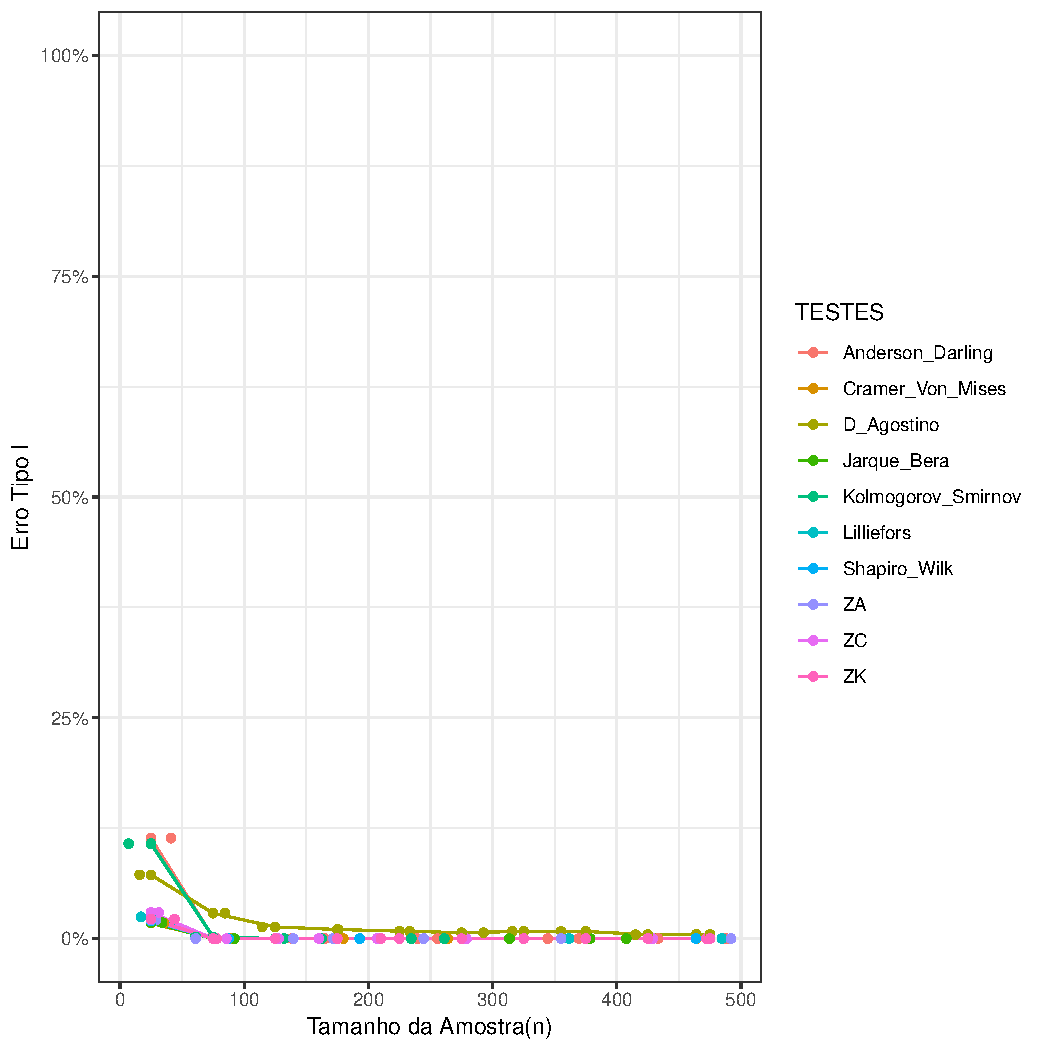
\includegraphics[width=\textwidth]{Distribuição cauchy/Erro Tipo I/erro_tipo_I_cauchy_500.pdf}
        \caption{Tamanho amostral \(n = 500\)}
        \label{fig:cauchy_500}
    \end{subfigure}
    \hfill
    \begin{subfigure}[b]{0.45\textwidth}
        \centering
        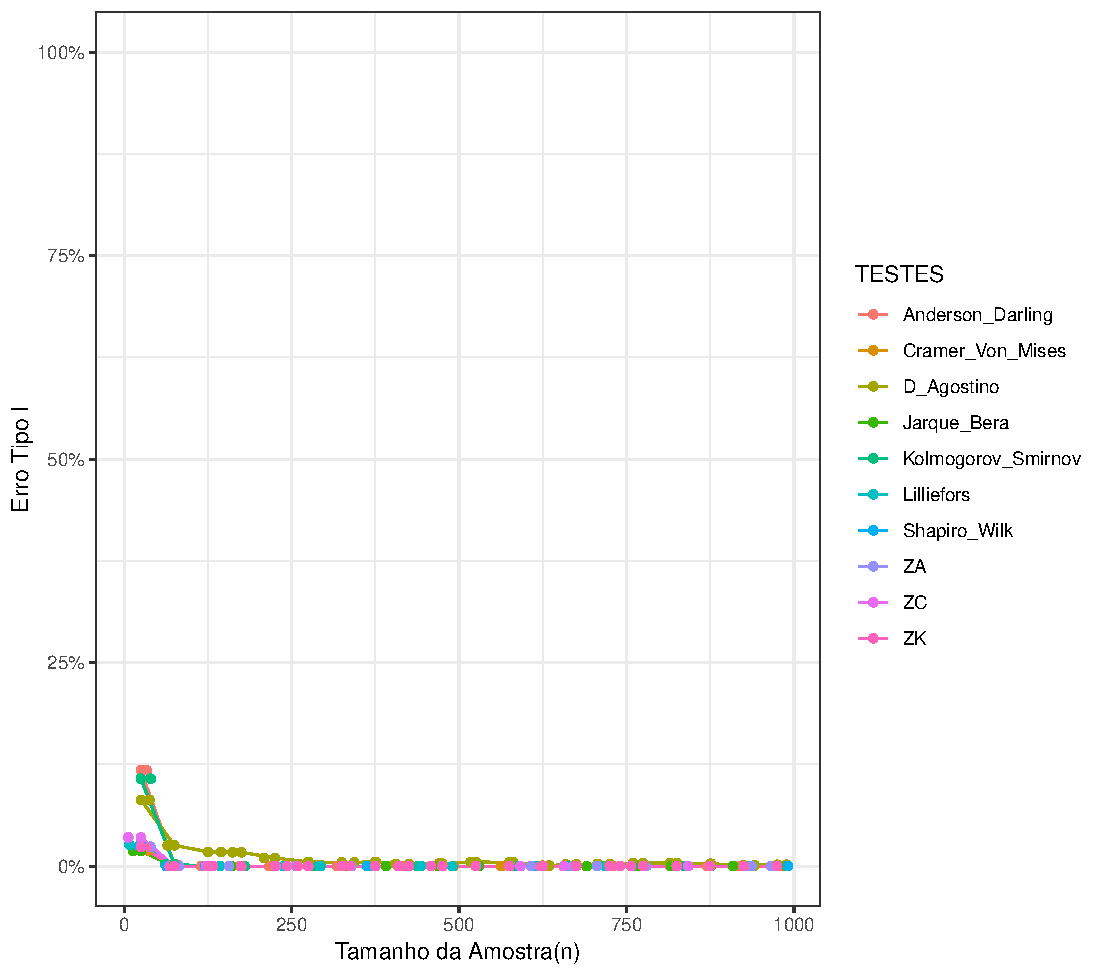
\includegraphics[width=\textwidth]{Distribuição cauchy/Erro Tipo I/erro_tipo_I_cauchy_1000.pdf}
        \caption{Tamanho amostral \(n = 1000\)}
        \label{fig:cauchy_1000}
    \end{subfigure}
\end{figure}

%%%%%%%%%% Poder do Teste -> Distribuição Cauchy %%%%%%%%%%
\begin{figure}[H]
    \centering
    \caption{Comparação do Poder do Teste dos testes AD, CM, DG, LL, JB, KS, ZA, ZC e ZK em função do tamanho amostral para a \textbf{Distribuição} \(\textbf{Cauchy}(0, 1)\).}
    \label{fig:poder_teste_dist_cauchy}
    
    % Primeira linha
    \begin{subfigure}[b]{0.45\textwidth}
        \centering
        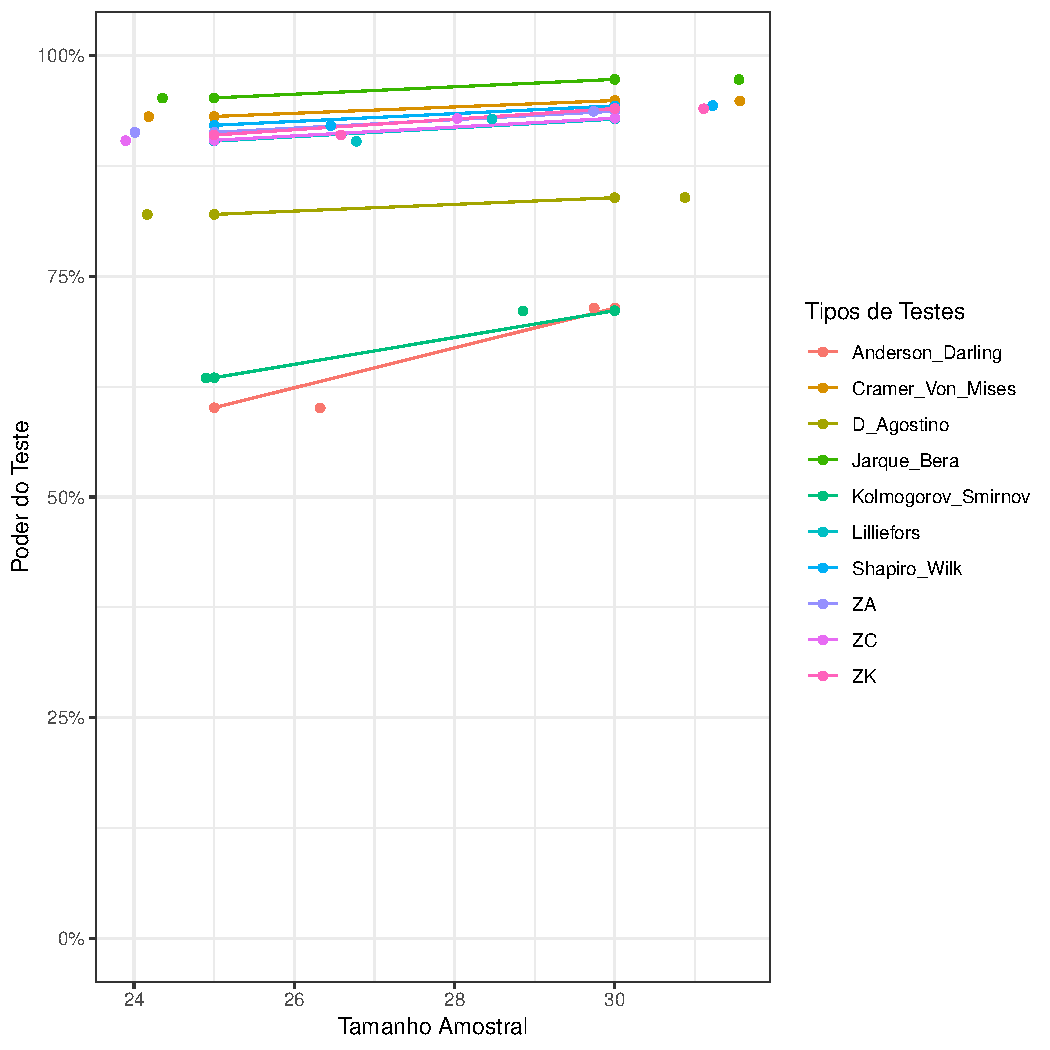
\includegraphics[width=\textwidth]{Distribuição Cauchy/Poder do Teste/poder_teste_cauchy_30.pdf}
        \caption{Tamanho amostral \(n = 30\)}
        \label{fig:cauchy_poder_30}
    \end{subfigure}
    \hfill
    \begin{subfigure}[b]{0.45\textwidth}
        \centering
        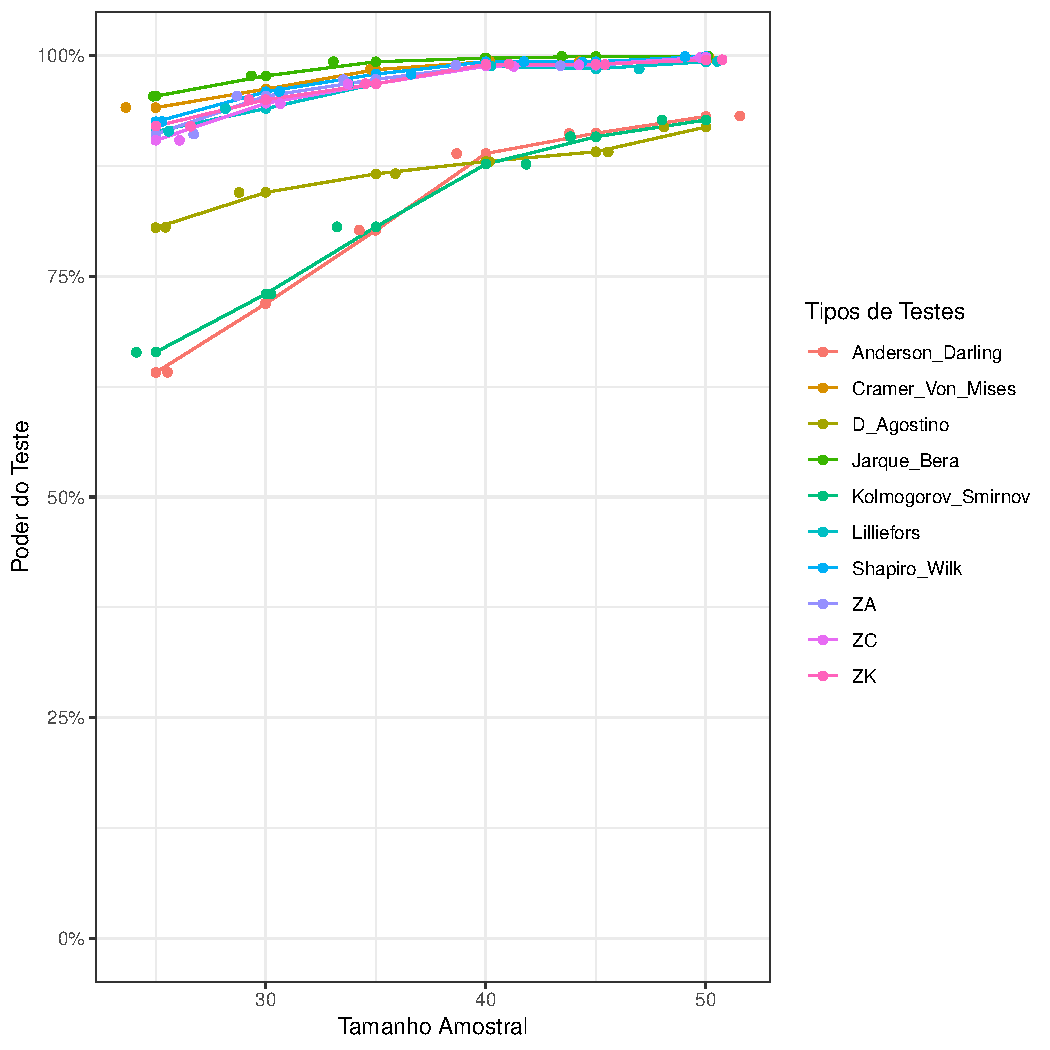
\includegraphics[width=\textwidth]{Distribuição Cauchy/Poder do Teste/poder_teste_cauchy_50.pdf}
        \caption{Tamanho amostral \(n = 50\)}
        \label{fig:cauchy_poder_50}
    \end{subfigure}
    
    % Segunda linha
    \vspace{0.5cm} % Espaçamento entre linhas
    \begin{subfigure}[b]{0.45\textwidth}
        \centering
        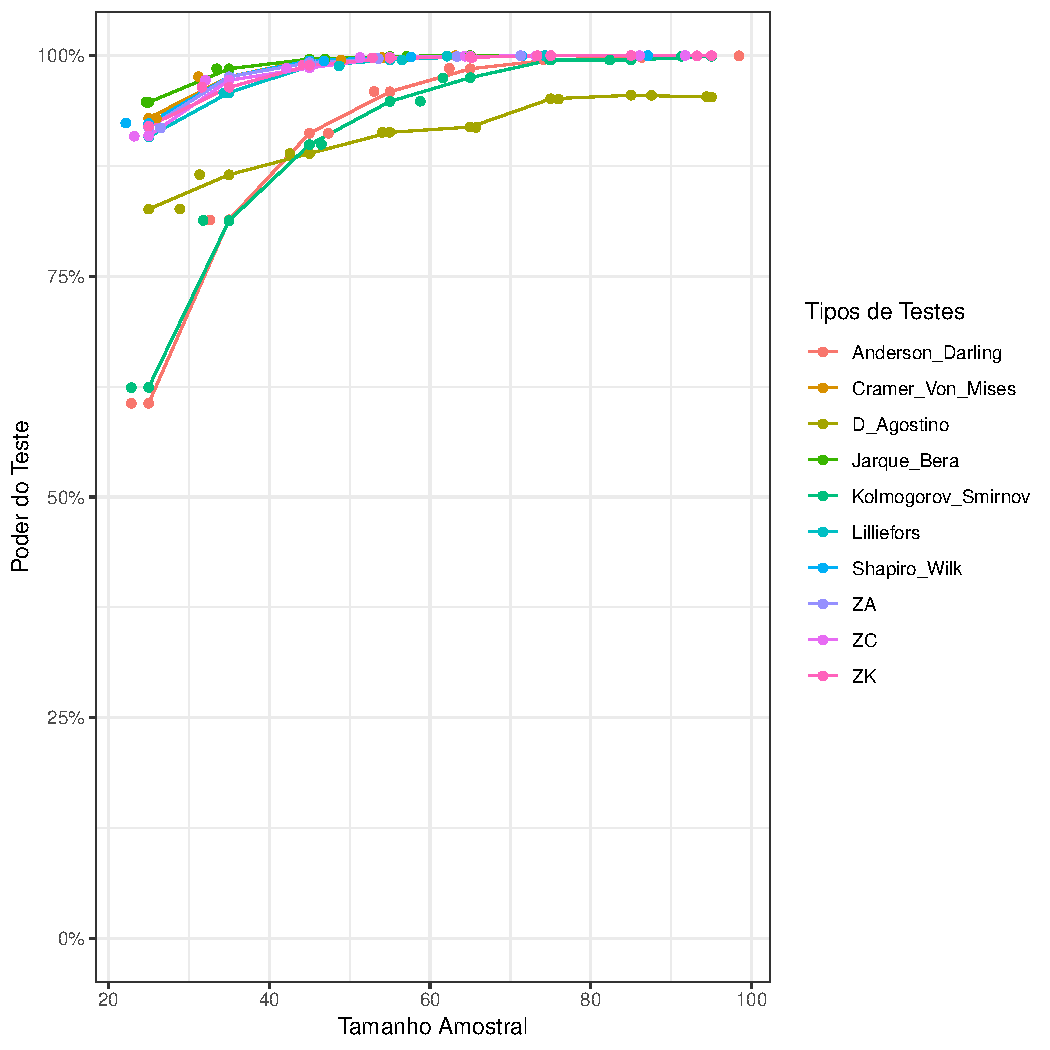
\includegraphics[width=\textwidth]{Distribuição cauchy/Poder do Teste/poder_teste_cauchy_100.pdf}
        \caption{Tamanho amostral \(n = 100\)}
        \label{fig:cauchy_poder_100}
    \end{subfigure}
    \hfill
    \begin{subfigure}[b]{0.45\textwidth}
        \centering
        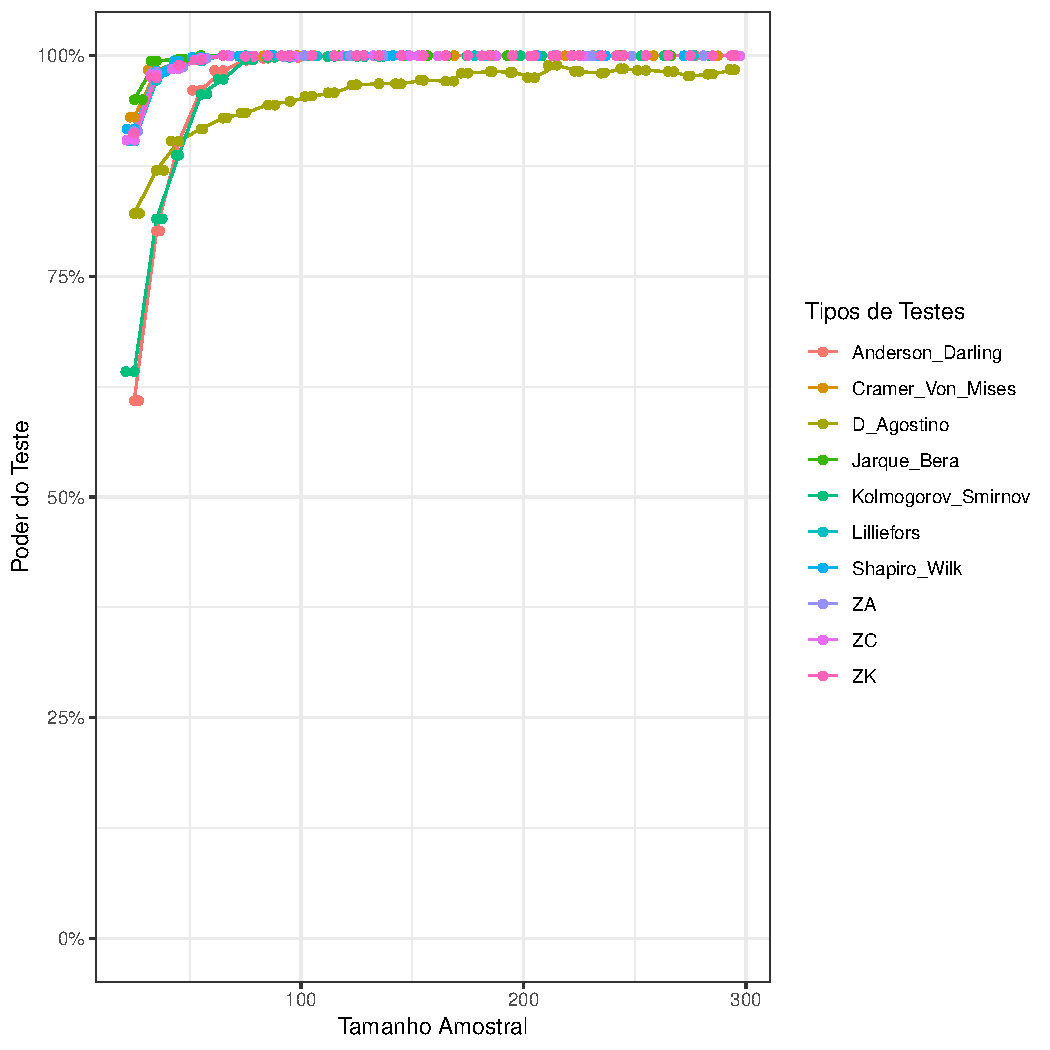
\includegraphics[width=\textwidth]{Distribuição Beta/Poder do Teste/poder_teste_cauchy_300.pdf}
        \caption{Tamanho amostral \(n = 300\)}
        \label{fig:cauchy_poder_300}
    \end{subfigure}
    
    % Terceira linha
    \vspace{0.5cm} % Espaçamento entre linhas
    \begin{subfigure}[b]{0.45\textwidth}
        \centering
        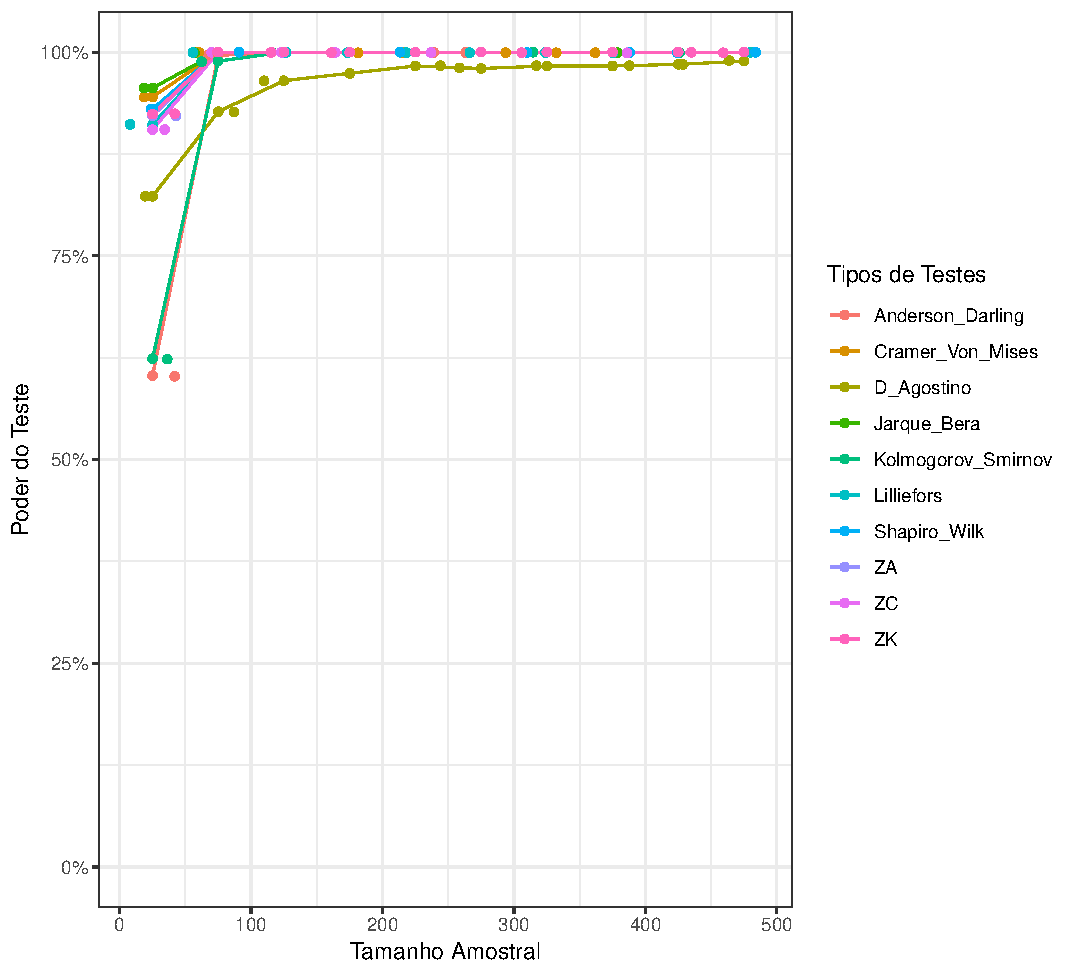
\includegraphics[width=\textwidth]{Distribuição Beta/Poder do Teste/poder_teste_cauchy_500.pdf}
        \caption{Tamanho amostral \(n = 500\)}
        \label{fig:cauchy_poder_500}
    \end{subfigure}
    \hfill
    \begin{subfigure}[b]{0.45\textwidth}
        \centering
        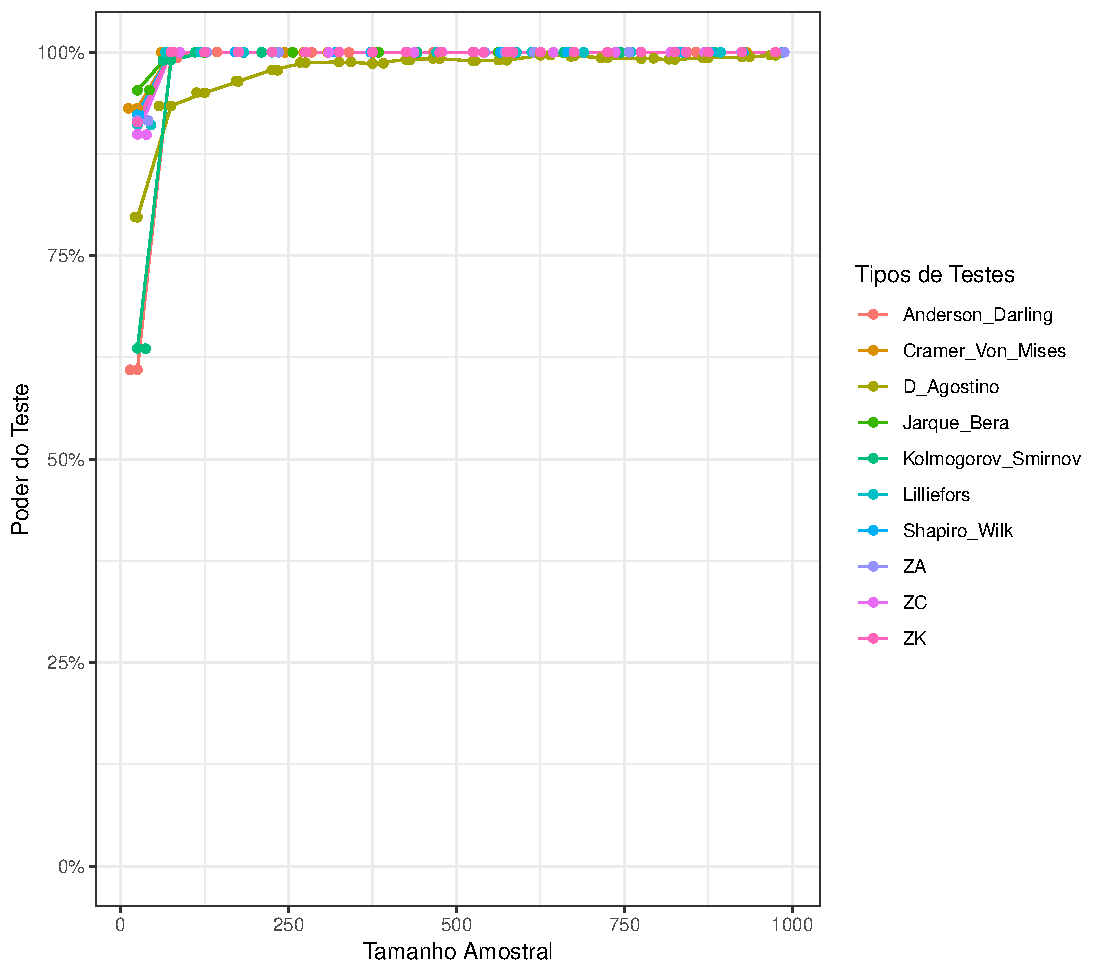
\includegraphics[width=\textwidth]{Distribuição Beta/Poder do Teste/poder_teste_cauchy_1000.pdf}
        \caption{Tamanho amostral \(n = 1000\)}
        \label{fig:cauchy_poder_1000}
    \end{subfigure}
\end{figure}

%%%%%%%%%%%%%%%%%%%%%%%%%%%%%%%%%%%%%%%%%%%%%%%%%%%%%%%%%%%%%%%%%%%%%%%%%%%%%%%%%%%%%%%%%%%%




\section{Considerações Finais}

Para dados de distribuição normal, os testes avaliados foram exatos, controlando a taxa de erro tipo I. Em relação ao poder, o desempenho dos testes foi afetado pelo tamanho da amostra e pelo tipo da distribuição. Todos se tornaram mais poderosos à medida que se aumentou o tamanho amostral. 


\section*{Referências}

\begin{flushleft}

\noindent ANDERSON, T. W.; DARLING, D. A. Asymptotic theory of certain goodness of fit criteria based on stochastic processes. {\it The Annals of Mathematical Statistics}, JSTOR, p. 193–212, 1952.\newline
    
\noindent DARLING, D. A. The Kolmogorov-Smirnov, Cramer-von Mises tests. {\it The Annals of Mathematical Statistics}, JSTOR, v. 28, n. 4, p. 823–838, 1957.\newline


\noindent Dallal, G.E. and Wilkinson, L. (1986): An analytic approximation to the distribution of Lilliefors’test for normality. The American Statistician, 40, 294–296.\newline


\noindent D'Agostino, Ralph B.; Pearson, E. S. (1973). "Tests for Departure from Normality. Empirical Results for the Distributions of b2 and b1. Biometrika. 60(3): 613–622
\newline
    
\noindent DUFOUR, J. - M. et al. Simulation-based finite sample normality tests in linear regressions. {\it The Econometrics Journal}, Wiley Online Library, v. 1, n. 1, p. 154–173, 1998.\newline
    
\noindent JARQUE, C. M.; BERA, A. K. Efficient tests for normality, homoscedasticity and serial independence of regression residuals. {\it Economics Letters}, Elsevier, v. 6, n. 3, p. 255–259, 1980.\newline

\noindent JIN ZHANG, 2002. "Powerful goodness‐of‐fit tests based on the likelihood ratio," Journal of the Royal Statistical Society Series B, Royal Statistical Society, vol. 64(2), pages 281-294, May.\newline

\noindent LILLIEFORS, H. W. On the Kolmogorov-Smirnov test for normality with mean and variance unknown. {\it Journal of the American Statistical Association}, Taylor \& Francis, v. 62, n. 318, p. 399–402, 1967.\newline

\noindent MEYER, Paul, L. – Probabilidade: Aplicação à Estatística – Ed. Livro Técnico, 1987. \newline
    
\noindent R CORE TEAM (2024). {\it R: A language and environment for statistical computing}. R Foundation for Statistical Computing, Vienna, Austria. Disponível em: \url{http://www.R-project.org/}.\newline

\noindent SHAPIRO, S. S.; WILK, M. B. An analysis of variance test for normality (complete samples). {\it Biometrika}, JSTOR, v. 52, n. 3/4, p. 591–611, 1965.\newline

\noindent STEPHENS, M.A. (1974): EDF statistics for goodness of fit and some comparisons. Journal of the American Statistical Association, 69, 730–737.\newline
    
\noindent STEPHENS, M. A. The Anderson-Darling statistic. {\it Stanford University}, 1979.\newline

\noindent STEPHENS, M.A. (1986): Tests based on EDF statistics. In: D’Agostino, R.B. and Stephens, M.A., eds.: Goodness-of-Fit Techniques. Marcel Dekker, New York.\newline

\noindent THODE JUNIOR, HC. Testing for Normality, New York: M Decker, 2002, 154p.


\end{flushleft}

	
	
	
\end{document}

